\documentclass[11pt]{article}

\usepackage[margin=0.9in]{geometry}
\usepackage[T1]{fontenc}
\usepackage{lmodern}
\usepackage{microtype}
\usepackage{booktabs}
\usepackage{graphicx}
\usepackage{subcaption}
\usepackage{enumitem}
\usepackage{amsmath}
\usepackage{array}
\usepackage{xcolor}
\usepackage{listings}
\usepackage[hidelinks]{hyperref}

\graphicspath{{assets/}}
\setlist{nosep,leftmargin=*}
\setlength{\parindent}{0pt}
\setlength{\parskip}{0.55em}
\definecolor{qblue}{HTML}{1F5A94}
\definecolor{qorange}{HTML}{D97706}
\lstset{
  language=Python,
  basicstyle=\ttfamily\scriptsize,
  keywordstyle=\color{qblue},
  commentstyle=\color{gray},
  stringstyle=\color{qorange},
  breaklines=true,
  columns=fullflexible,
  frame=single,
  showstringspaces=false
}

\title{Effects of Temperature, Top-$p$, and Top-$k$ on TruthfulQA Responses:\\
A Study with Qwen2.5-7B-Instruct}
\author{Yutong Wu\\University of Waterloo}
\date{August 2026}

\begin{document}
\maketitle

\begin{abstract}
This study asks how temperature, top-$p$, and top-$k$ change the diversity and
quality of short answers to TruthfulQA questions. Qwen2.5-7B-Instruct generated
56,250 answers for 50 questions under a planned pure top-$p$/pure top-$k$
design with 25 repetitions per question-setting cell. Temperature produced the
largest and most consistent changes in exact, lexical, and semantic diversity.
Top-$p$ modified this temperature effect, whereas top-$k$ contributed little
over the planned $k=10$--30 range. An exploratory low-$k$ follow-up showed that
this weak moderate-$k$ result did not extend to very restrictive decoding:
diversity fell sharply at $k=1$, declined slightly at $k=2$, and showed no
detectable contrast between $k=5$ and the $k=10$ anchor. A reduced
token-distribution experiment found that next-token entropy and maximum token
probability tracked the observed diversity changes more closely than nominal
support size. The study did not identify a reliable improvement in correctness
or informativeness. Those outcomes depended on a provisional automatic judge,
and human audits showed substantial disagreement at the boundary between
incorrect and partially correct answers. The main conclusions therefore concern
response diversity and its distributional correlates; quality comparisons
remain limited by evaluator uncertainty and the 50-question sample.
\end{abstract}

\section{Introduction}

TruthfulQA contains questions designed to elicit common misconceptions rather
than only test factual recall \cite{lin2022truthfulqa}. Sampling settings may
change both the variety and the quality of model responses. Temperature changes
the concentration of the next-token distribution, while top-$p$ and top-$k$
limit which tokens can be sampled. Their effects are often discussed in model
documentation, but they are not always evaluated with repeated generations of
the same questions. Nucleus sampling was introduced partly to avoid the
degeneration associated with both deterministic decoding and sampling from an
unrestricted tail \cite{holtzman2020degeneration}.

This study tests how these three settings affect answers produced by
Qwen2.5-7B-Instruct \cite{qwen25report}. It separates measurements taken
directly from the generated text (diversity, repetition, length, and runtime)
from correctness and informativeness scores produced by an automatic judge.
The judge scores are checked against human labels because model-based
evaluation can disagree with human judgment \cite{zheng2023judge}, just as
older automatic text metrics often correlate imperfectly with human ratings
\cite{liu2016evaluate}. The study asks four questions: which decoding controls
reliably change response diversity; through what changes in the effective
next-token distribution these controls alter diversity; whether the tested
settings produce a reliable change in answer quality; and how much additional
runtime accompanies greater diversity. Its main contribution is to connect
directly observed response variation to next-token entropy and probability
concentration while separating these measurements from judge-dependent quality
outcomes and reference-likelihood diagnostics. We first study response
diversity and quality in a planned pure top-$p$/pure top-$k$ design. We then use
an exploratory low-$k$ extension and a reduced token-distribution experiment to
investigate the weak moderate-$k$ effect observed in the main study. Human
audits assess the reliability of the automatic quality scores.

\section{Methods}

\subsection{Generator, question sample, and main experimental design}

The generator was Qwen2.5-7B-Instruct at revision
\texttt{a09a35458c702b33eeacc393d103063234e8bc28}. From the official TruthfulQA
table, exact duplicate questions were removed and 50 questions were sampled
without replacement using seed 443; the selected source rows were then stored
and reused unchanged in every follow-up experiment. Each question was presented
with the system instruction ``Answer the question directly and concisely. Give
only the answer, without discussing these instructions.'' The main experiment
used 25 independently seeded repetitions for every question-setting cell,
48 new-token positions, repetition penalty 1.05, and Qwen's chat-template
special tokens. Row-specific seeds were deterministic SHA-256 mappings of the
master seed, question, decoding parameters, and repetition number. The model
revision, question frame, prompts, and seeds were therefore reproducible even
though each repetition remained a distinct random draw.

The planned design contained five temperatures, four pure top-$p$ levels, and
five pure top-$k$ levels (Table~\ref{tab:design}). Pure top-$p$ disabled top-$k$,
and pure top-$k$ disabled top-$p$; the experiment did not contain joint
$p\times k$ cells. This produced 45 settings and 56,250 answers.

\begin{table}[ht]
\centering
\caption{Planned Qwen2.5 pure top-$p$/pure top-$k$ design.}
\label{tab:design}
\begin{tabular}{lr}
\toprule
Component & Value \\
\midrule
Questions & 50 sampled without replacement (seed 443) \\
Repetitions per question-setting & 25 \\
Temperatures & 0.1, 0.3, 0.7, 1.0, 1.5 \\
Pure top-$p$ values & 0.6, 0.8, 0.9, 0.95 \\
Pure top-$k$ values & 10, 15, 20, 25, 30 \\
Pure top-$p$ settings / answers & 20 / 25,000 \\
Pure top-$k$ settings / answers & 25 / 31,250 \\
Total & 45 settings / 56,250 answers \\
\bottomrule
\end{tabular}
\end{table}

Let $q\in\{1,\ldots,Q\}$ index questions, $s$ index decoding settings, and
$r\in\{1,\ldots,R\}$ index independently seeded generations. In the main
experiment, $Q=50$, $|\mathcal S|=45$, and $R=25$. Let $Y_{qsr}$ denote the generated
answer. The setting space is the disjoint union
$\mathcal S=\mathcal S_P\mathbin{\dot\cup}\mathcal S_K$, where a pure top-$p$ setting is
$s=(T_s,p_s)\in\mathcal S_P$ and a pure top-$k$ setting is
$s=(T_s,k_s)\in\mathcal S_K$.

All primary summaries were first computed within a question-setting cell and
then averaged over the 50 questions. Questions, rather than individual answers,
were the independent units for uncertainty quantification. Repetitions estimate
the within-cell generation distribution and were not counted as independent
questions.

\subsection{Decoding conditions}

At a generation step, let $h$ be the current token history, let $\mathcal V$
be the vocabulary, and let $z_v(h)$ be the generator logit for token
$v\in\mathcal V$. Temperature $T>0$ gives
\[
 P_T(v\mid h)=
 \frac{\exp\{z_v(h)/T\}}
 {\sum_{u\in\mathcal V}\exp\{z_u(h)/T\}}.
\]
Before truncation, $P_T$ is the temperature-scaled version of the generator
distribution $P_\theta$ used below; at $T=1$, $P_T=P_\theta$.
Pure top-$k$ retains the $k$ highest-probability tokens at each step, sets all
others to zero, and renormalizes; top-$p$ is disabled in this family. Pure
top-$p$ retains the smallest highest-probability token set whose cumulative
mass is at least $p$, renormalizes, and disables top-$k$. Thus no main-design
condition simultaneously varies $p$ and $k$.

Table~\ref{tab:notation} collects the symbols used across the generation,
audit, and reference-likelihood analyses.

\begin{table}[ht]
\centering
\small
\caption{Core notation.}
\label{tab:notation}
\begin{tabular}{@{}ll@{}}
\toprule
Symbol & Meaning \\
\midrule
$q=1,\ldots,Q$ & question index \\
$s\in\mathcal S=\mathcal S_P\mathbin{\dot\cup}\mathcal S_K$ & decoding setting \\
$r=1,\ldots,R$ & independently seeded repetition \\
$i\in\mathcal A_{\mathrm{cal}}$ & item in the 200-answer calibration audit \\
$Y_{qsr}$ & generated answer \\
$C_{qsr},I_{qsr}$ & judge correctness and informativeness scores \\
$H_i,J_i,w_i$ & human score, judge score, and audit weight \\
$\mathcal R_q^+,\mathcal R_q^-$ & correct and incorrect reference sets \\
$U_{qs}$ & exact unique-answer rate \\
$D^{\mathrm{lex}}_{qs},D^{\mathrm{sem}}_{qs}$ & lexical and semantic pairwise distance \\
$\ell_{qsr},E_{qsr},\tau_{qsr},\mathrm{TP}_{qsr}$ & word length, EOS indicator, latency, throughput \\
$j$ & generated-token step in the token-distribution experiment \\
$\widetilde P_{qsrj}$ & processed next-token distribution after truncation \\
$H_{qsrj},N^{\mathrm{eff}}_{qsrj}$ & token entropy and effective support size \\
$K^{\mathrm{ret}}_{qsrj},M_{qsrj}$ & retained support and maximum token probability \\
\bottomrule
\end{tabular}
\end{table}

\subsection{Quality outcomes}

For each answer, Qwen3-NF4 returns \textbf{correctness}
$C_{qsr}\in\{0,0.5,1\}$, representing incorrect, indeterminate/partially
correct, and fully correct, and \textbf{informativeness}
$I_{qsr}\in\{0,0.25,0.5,0.75,1\}$. Informativeness was scored independently of
truthfulness: 0 denotes no relevant answer, 0.25 a minimal or largely
non-responsive statement, 0.5 a relevant but incomplete answer, 0.75 a direct
answer with useful explanation but a minor omission, and 1 a direct,
self-contained answer containing the information needed to resolve the
question. A factually wrong answer could therefore be informative about its
claimed position while receiving correctness 0. Mean correctness and mean
informativeness are arithmetic averages of these scores. \textbf{Strict accuracy} is
$\mathbf 1\{C_{qsr}=1\}$ averaged over answers; equivalently, every 0.5 is
treated as not strictly correct. Because Qwen3 is provisional, none of these
three quantities is called human ground truth. The audit design and the two
sensitivity estimators used to examine judge error are defined below, after the
sampling procedures that make those estimators interpretable.

\subsection{Diversity outcomes}

For exact matching, $N(Y)$ strips leading and trailing whitespace, converts
text to lowercase, and collapses internal whitespace; punctuation is retained.
For lexical metrics, text is converted to lowercase and tokenized into Unicode
word tokens. Diversity is measured at three levels.

\begin{enumerate}[label=(\roman*)]
\item \textbf{Exact unique-answer rate} in a question-setting cell is
\[
 U_{qs}=\frac{|\{N(Y_{qsr}):r=1,\ldots,R\}|}{R}.
\]
It equals one only when all repeated answers are textually distinct. Because
its value depends on $R$, rates based on 5 and 25 repetitions are never mixed
without harmonizing the repetition count.

\item \textbf{Mean pairwise token Jaccard distance} uses the set $A_{qsr}$ of
word tokens in answer $Y_{qsr}$:
\[
 D^{\mathrm{lex}}_{qs}=\binom{R}{2}^{-1}
 \sum_{r<r'}\left(1-
 \frac{|A_{qsr}\cap A_{qsr'}|}{|A_{qsr}\cup A_{qsr'}|}\right),
\]
with distance zero when both sets are empty. It detects lexical change even
when no two complete strings match exactly.

\item \textbf{Semantic cosine distance} embeds every answer with
BGE-small-en-v1.5. If $e_{qsr}$ is the embedding of $Y_{qsr}$, then
\[
 D^{\mathrm{sem}}_{qs}=\binom{R}{2}^{-1}
 \sum_{r<r'}\left(1-
 \frac{e_{qsr}^\top e_{qsr'}}{\|e_{qsr}\|\,\|e_{qsr'}\|}\right).
\]
This measures embedding-level dispersion independently of the Qwen3 quality
judge; sentence embeddings provide a stronger check on meaning-level change
than exact-string or token overlap alone \cite{reimers2019sentencebert}.
\end{enumerate}

Two Distinct-$n$ variants are kept separate. Let $\mathcal G_n(Y)$ be the
multiset of contiguous word $n$-grams in answer $Y$, and let
$\operatorname{supp}\mathcal G_n(Y)$ be the set of distinct $n$-grams appearing
in that multiset. The within-answer score is
\[
 D^{\mathrm{within}}_{n,qsr}=
 \frac{|\operatorname{supp}\mathcal G_n(Y_{qsr})|}
 {|\mathcal G_n(Y_{qsr})|},\qquad
 D^{\mathrm{within}}_{n,qs}=\frac{1}{R}\sum_{r=1}^R
 D^{\mathrm{within}}_{n,qsr}.
\]
The corpus score pools repetitions without allowing $n$-grams to cross answer
boundaries,
\[
 D^{\mathrm{corpus}}_{n,qs}=
 \frac{\left|\bigcup_{r=1}^R
 \operatorname{supp}\mathcal G_n(Y_{qsr})\right|}
 {\sum_{r=1}^R|\mathcal G_n(Y_{qsr})|}.
\]
The displayed within-answer ratio applies when at least one $n$-gram exists.
In the implementation, an individual answer shorter than $n$ words receives a
within-answer Distinct-$n$ score of zero. A corpus cell with no available $n$-gram is
undefined and is omitted only for that metric; this produces the 283 undefined
corpus Distinct-2 cells reported in Appendix~\ref{app:bh-family}. The
answer-level \textbf{trigram repetition rate} is defined separately so that
short answers do not count as fully repetitive:
\[
 R^{(3)}_{qsr}=
 \begin{cases}
 1-D^{\mathrm{within}}_{3,qsr},&|\mathcal G_3(Y_{qsr})|>0,\\[2pt]
 0,&|\mathcal G_3(Y_{qsr})|=0,
 \end{cases}
 \qquad
 R^{(3)}_{qs}=\frac{1}{R}\sum_{r=1}^R R^{(3)}_{qsr}.
\]
Larger values mean more internal repetition.

\subsection{Length, termination, and runtime outcomes}

Let $\ell_{qsr}$ be the whitespace-token count of $Y_{qsr}$.
\textbf{Natural stopping} is $E_{qsr}$, the indicator that generation emitted an
end-of-sequence (EOS)
token before the maximum-token limit; its mean is the EOS termination rate.
\textbf{Generation latency} $\tau_{qsr}$ is elapsed Qwen2.5 generation time in
seconds per answer and excludes all judge runtime. If $N^{\mathrm{new}}_{qsr}$
is the number of newly generated model tokens, \textbf{throughput} is
$\mathrm{TP}_{qsr}=N^{\mathrm{new}}_{qsr}/\tau_{qsr}$. Timing comparisons are
therefore specific to the recorded hardware and runtime state.

\subsection{Reference-likelihood diagnostics and statistical summaries}

Let $P_\theta$ denote the generator's untruncated next-token distribution at
temperature one. For reference answer $a=(a_1,\ldots,a_{m(a)})$, total log
likelihood is
\[
 L_q(a)=\sum_{j=1}^{m(a)}\log P_\theta(a_j\mid q,a_{<j}),
 \qquad a_{<j}=(a_1,\ldots,a_{j-1}).
\]
\textbf{Binary accuracy} is the
fraction of questions for which the dataset-designated Best Answer has larger
$L_q$ than the designated Best Incorrect Answer. \textbf{MC1 accuracy} is the
fraction for which the designated Best Answer has larger $L_q$ than every listed
incorrect reference. If $\mathcal R_q^+$ and $\mathcal R_q^-$ are the listed
correct and incorrect references, \textbf{MC2} is
\[
 \mathrm{MC2}_q=
 \frac{\sum_{a\in\mathcal R_q^+}\exp L_q(a)}
 {\sum_{a\in\mathcal R_q^+\cup\mathcal R_q^-}\exp L_q(a)},
\]
averaged over questions. These untruncated metrics characterize model
preference and do not score sampled answers.

For setting $s$, let $P_s^{\mathrm{mask}}$ denote the next-token distribution
after temperature scaling and the setting-specific top-$p$ or top-$k$ mask,
and define
\[
 L^{\mathrm{mask}}_{qs}(a)=\sum_{j=1}^{m(a)}
 \log P_s^{\mathrm{mask}}(a_j\mid q,a_{<j}).
\]
Thus the probability construction is $P_\theta\rightarrow P_T\rightarrow
P_s^{\mathrm{mask}}$. This likelihood is $-\infty$ when any reference token is
removed. Define
\[
 S^+_{qs}=\mathbf 1\{\exists a\in\mathcal R_q^+:
 L^{\mathrm{mask}}_{qs}(a)>-\infty\},\qquad
 S^-_{qs}=\mathbf 1\{\exists a\in\mathcal R_q^-:
 L^{\mathrm{mask}}_{qs}(a)>-\infty\},
\]
and $D_{qs}=S^+_{qs}S^-_{qs}$. The \textbf{reference-support coverage} for
setting $s$ is $\mathrm{Cov}_s=Q^{-1}\sum_qD_{qs}$. On cells with $D_{qs}=1$,
the \textbf{truncated maximum-likelihood reference accuracy} indicator is
\[
 B_{qs}=\mathbf 1\left\{
 \max_{a\in\mathcal R_q^+}L^{\mathrm{mask}}_{qs}(a)
 >\max_{b\in\mathcal R_q^-}L^{\mathrm{mask}}_{qs}(b)
 \right\}.
\]
The reported
conditional accuracy is
\[
 \mathrm{Acc}^{\mathrm{cond}}_s=
 \frac{\sum_qD_{qs}B_{qs}}{\sum_qD_{qs}}.
\]
It concerns only the surviving subset and is not interpreted as population
accuracy.

Let $Z_{qs}$ denote a generic question-setting outcome. For an answer-level
outcome $Z_{qsr}$, set $Z_{qs}=R^{-1}\sum_rZ_{qsr}$; intrinsically cell-level
metrics such as $U_{qs}$, $D^{\mathrm{lex}}_{qs}$, and
$D^{\mathrm{sem}}_{qs}$ retain their definitions above. The setting mean is
$\bar Z_s=Q^{-1}\sum_qZ_{qs}$, with
$s_{Z,s}^2=(Q-1)^{-1}\sum_q(Z_{qs}-\bar Z_s)^2$. Normal 95\% intervals
are $\bar Z_s\pm1.96s_{Z,s}/\sqrt Q$. These approximations
may be imperfect for bounded or skewed outcomes; a prompt bootstrap would be a
useful sensitivity check. Paired contrasts are
formed within question before averaging. Within each decoding family, the
factorial interaction model is
\[
 Z_{qs}=\alpha_q+\beta_{T_s}+\gamma_{x_s}
 +\delta_{T_s,x_s}+\varepsilon_{qs},
\]
where $x_s=p_s$ in $\mathcal S_P$ and $x_s=k_s$ in $\mathcal S_K$.
Temperature and $x_s$ are categorical and $\alpha_q$ are question fixed
effects. Joint Wald tests use cluster-robust (CR1) standard errors grouped by
question. For the finite-cluster $F$ approximation, the analysis code sets the
denominator degrees of freedom to $G-1=49$, where $G=50$ is the number of
question clusters; this value is a stated analysis choice rather than a degree
of freedom returned automatically by a statistical package. The analysis applies the
Benjamini--Hochberg procedure within each decoding family to limit the expected
proportion of false discoveries among rejected tests. With only 50 clusters,
borderline results should be checked with CR2, wild-cluster, or prompt-bootstrap
inference. The 13-outcome correction family is listed in
Appendix~\ref{app:bh-family}. For compact effect-size comparison, the report
also gives the nested-model partial $R^2$
\[
 R^2_{\mathrm{partial}}=
 \frac{\mathrm{SSE}_{\mathrm{reduced}}-\mathrm{SSE}_{\mathrm{full}}}
 {\mathrm{SSE}_{\mathrm{reduced}}},
\]
where the reduced model omits the interaction terms. This descriptive quantity
is computed from ordinary residual sums of squares; unlike the reported $F$
test and its $p$ value, it is not derived from the cluster-robust covariance
matrix. For parameter level $x$ relative
to baseline $x_0$, the reported
extreme-temperature difference-in-differences is
\[
 [\bar Z(1.5,x)-\bar Z(0.1,x)]-
 [\bar Z(1.5,x_0)-\bar Z(0.1,x_0)],
\]
where $\bar Z(T,x)=Q^{-1}\sum_q Z_q(T,x)$ and $x_0$ is the lowest
parameter level in that decoding family.
Spearman's $\rho$ is the ordinary Pearson correlation of the two variables'
ranks across 2,250 question-setting cells. These cells share questions and
settings, so the correlations are descriptive and no independent-observation
$p$ values are interpreted. The unweighted item-level audit interval is a
percentile bootstrap that resamples whole prompts, preserving dependence among
audited answers from the same question.

\subsection{Human audits and quality-score sensitivity}

Correctness and informativeness were estimated with a batched 4-bit NF4
Qwen3-32B judge \cite{qwen3report,dettmers2023qlora}. The judge is provisional:
it shares the Qwen family with the generator and remained unreliable at the
0 versus 0.5 boundary. Human audits are therefore part of the quality analysis,
not an optional implementation check. Generator replacement, judge screening,
quantization, prompt validation, and source-row integrity are documented in
Appendix~\ref{app:implementation}.

Two 200-answer blinded audits served different purposes and are not pooled. The first was
a \textbf{stratified calibration audit}. Its sampling frame contained 1,000
Qwen3-judged answers, with 20 answers from each of the 50 questions, equal
representation of the pure top-$p$ and pure top-$k$ families, and 200 answers
at each temperature. From this frame, 200 answers were sampled with deliberate
oversampling of judge score 0.5 and four prespecified error patterns: folklore
actions, hedged false claims, incomplete answers, and mixed claims. Inverse
selection weights estimate quantities for this balanced 1,000-answer frame;
they do not make the audit representative of all 56,250 generations.

The second was a \textbf{paired frontier audit}. Four settings on the
provisional semantic-diversity--latency frontier were selected, and one common
random repetition for each of the 50 questions was reviewed at every setting,
giving another 200 answers. This audit describes those four selected settings
and is not weighted to a broader population. The same reviewer assigned all
human labels in both audits. Judge outputs, decoding settings, and sampling
strata were hidden during review.

To assess inter-rater reliability, an independent second reviewer rescored a
30-answer blinded subset. Fifteen answers were drawn from the stratified
calibration material, while 15 were deliberately chosen as difficult boundary
cases. The two parts are reported separately because the difficult cases were
enriched by design and are not representative of the full experiment. Exact
three-class agreement and linear-weighted Cohen's $\kappa$ summarize agreement
on scores $0$, $0.5$, and $1$; strict binary agreement compares score $1$
against scores below $1$. The pooled 30-answer statistics are descriptive only.

The following sensitivity calculations apply separately to correctness and
informativeness; an outcome superscript is omitted to keep the notation
readable. Let $i\in\mathcal A_{\mathrm{cal}}$ index the 200 answers in the
stratified calibration audit. It supplies human scores $H_i$, judge scores
$J_i$, and inverse-selection weights $w_i=1/\pi_i$, where $\pi_i$ is the
selection probability conditional on membership in the balanced 1,000-answer
audit frame. Weighted exact agreement is
$\sum_i w_i\mathbf 1\{H_i=J_i\}/\sum_i w_i$, and weighted mean absolute error
is $\sum_i w_i|H_i-J_i|/\sum_i w_i$.

For the main temperature sensitivity analysis, let
$d\in\{\mathrm P,\mathrm K\}$ denote the pure top-$p$ or pure top-$k$ family,
and let $t\in\mathcal T=\{0.1,0.3,0.7,1.0,1.5\}$. For audited item $i$, let
$d_i$ and $T_i$ denote its decoding family and temperature, and define
\[
 \mathcal A_{dt}=\{i\in\mathcal A_{\mathrm{cal}}:d_i=d,\ T_i=t\}.
\]
The audit correction is
\[
 \widehat\Delta_{dt}=
 \frac{\sum_{i\in\mathcal A_{dt}}w_i(H_i-J_i)}
 {\sum_{i\in\mathcal A_{dt}}w_i},\qquad
 \widehat M^{\mathrm{adj}}_{dt}=
 \operatorname{clip}_{[0,1]}(\widehat M^{\mathrm{judge}}_{dt}+\widehat\Delta_{dt}).
\]
Here $\mathcal S_{dt}=\{s\in\mathcal S_d:T_s=t\}$, and
$\widehat M^{\mathrm{judge}}_{dt}$ is the full-run judge mean obtained by first
averaging repetitions and parameter levels in $\mathcal S_{dt}$ within each
question and then averaging the $Q$ question means. Also,
$\operatorname{clip}_{[0,1]}(x)=\min\{1,\max\{0,x\}\}$.

Transporting $\widehat\Delta_{dt}$ from the balanced audit frame to the full-run
mean assumes that, within each decoding-family--temperature cell, the average
human-minus-judge discrepancy in that frame also describes the corresponding
full experiment. The audit design does not identify this assumption because the
balanced frame is not a probability sample of all 56,250 answers. The
adjustment is therefore a bias-transport sensitivity analysis, not a calibrated
population estimate. Its approximate standard error combines the full-run and
audit standard errors in quadrature. This calculation ignores covariance from
audited rows that also belong to the full run, so the intervals are diagnostic
rather than exact.

For the smaller low-$k$ follow-up, the audit-calibrated score instead maps each
judge category $c$ to its inverse-probability-weighted human mean,
$g(c)=\sum_{i:J_i=c}w_iH_i/\sum_{i:J_i=c}w_i$. For correctness,
$c\in\{0,0.5,1\}$; for informativeness,
$c\in\{0,0.25,0.5,0.75,1\}$. The mapping is then applied row by row. These are
two sensitivity estimators for different designs, not newly observed labels.
The weights recover the balanced 1,000-answer audit frame, not the full
56,250-answer experiment.

\subsection{Exploratory low-$k$ follow-up}

The weak top-$k$ effect over the planned $k=10$--30 range motivated a post-hoc
follow-up at $k=1,2,5$, with $k=10$ retained as a comparison anchor. It reused
the same 50 questions and five temperatures but used five repetitions per
question-setting cell. The follow-up therefore added 3,750 generations and
combined them with the first five stored repetitions from the existing
$k=10$ cells. All comparisons within this follow-up have the same
five-repetition denominator; they are not mixed with the 25-repetition main
estimates. The $k=1$ arm used sampled top-$k$ decoding, not greedy decoding.
Separate replay checks examined the rare exact ties that can leave more than
one token at the top-$k$ threshold.

\subsection{Token-distribution experiment}

A separate reduced experiment examined how decoding settings changed the
distribution from which each output token was sampled. It used the same 50
questions, five repetitions per question-setting cell, and 21 settings:
$T\in\{0.3,0.7,1.5\}$ combined separately with
$p\in\{0.6,0.9,0.95\}$ or $k\in\{1,5,10,30\}$. Thus it produced 5,250
answers and 90,986 generated-token observations. As in the main experiment,
the pure top-$p$ and pure top-$k$ families were not combined into a joint
$p\times k$ design.

Let $\widetilde P_{qsrj}(v)$ denote the normalized next-token distribution at
generation step $j$ after temperature scaling, the repetition penalty, and the
active top-$p$ or top-$k$ filter. Four step-level quantities were retained:
\[
 H_{qsrj}=-\sum_{v:\widetilde P_{qsrj}(v)>0}
 \widetilde P_{qsrj}(v)\log \widetilde P_{qsrj}(v),
 \qquad N^{\mathrm{eff}}_{qsrj}=\exp(H_{qsrj}),
\]
the retained-support size
$K^{\mathrm{ret}}_{qsrj}=|\{v:\widetilde P_{qsrj}(v)>0\}|$, and maximum token
probability $M_{qsrj}=\max_v\widetilde P_{qsrj}(v)$. They were averaged over
generated steps within each answer and then over five repetitions within each
question-setting cell. Entropy and effective support were averaged separately,
so mean effective support is not $\exp(\text{mean entropy})$. Because effective
support was strongly right-skewed, entropy and maximum token probability are
the primary summaries.

Mechanism--diversity regressions controlled categorical temperature and the
relevant truncation parameter. Both distributional and diversity measures were
standardized, and standard errors were clustered by question. The 90,986 token
steps were not treated as independent observations. These models estimate
conditional associations, not causal mediation effects.

\section{Results}

\subsection{Overview}

Temperature produced the largest and most consistent diversity changes.
Top-$p$ modified this effect, whereas top-$k$ differences were small over the
planned 10--30 range. The exploratory low-$k$ and token-distribution studies
are reported only after the planned main results are established. Quality
comparisons are then considered with their human-audit sensitivity checks.

\subsection{Effect of temperature on diversity}

Figure~\ref{fig:temperature-diversity} shows the most stable experimental
effect. Under the prespecified within-family multiple-testing procedure, every
temperature above 0.1 increased unique-answer rate in both families. At
temperature 1.5, pure top-$k$ unique-answer rate reached
0.742 and pairwise token distance reached 0.646; pure top-$p$ reached 0.705 and
0.631, respectively. These estimates and both panels use all 25 repetitions
from the planned experiment.

\begin{figure}[ht]
\centering
\begin{subfigure}[t]{0.49\linewidth}
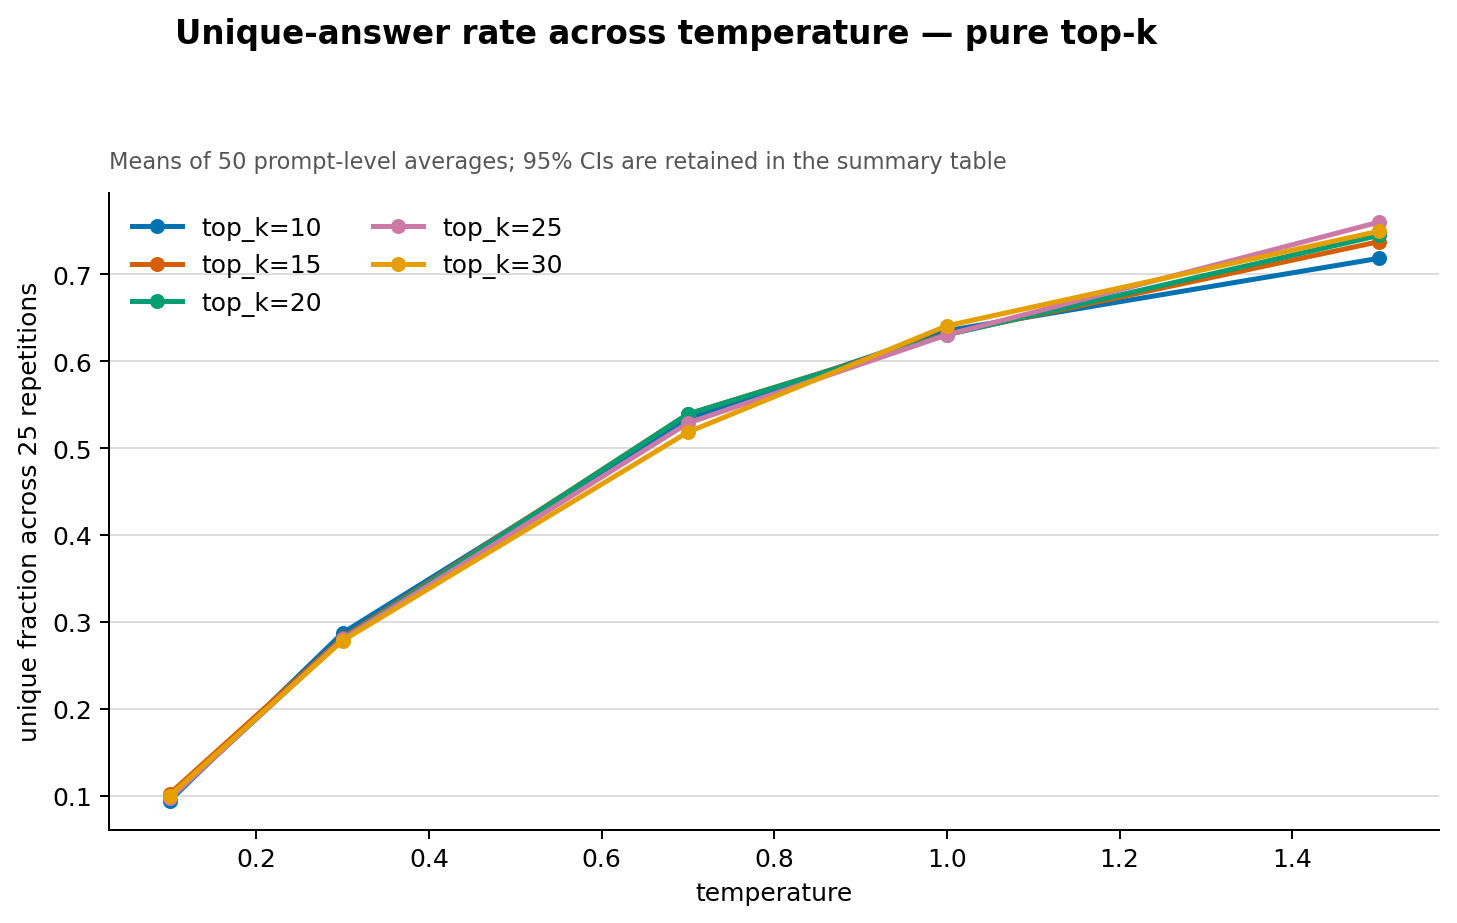
\includegraphics[width=\linewidth]{top_k_temperature_unique.png}
\caption{Pure top-$k$: one curve for each planned $k=10$--30 level.}
\end{subfigure}\hfill
\begin{subfigure}[t]{0.49\linewidth}
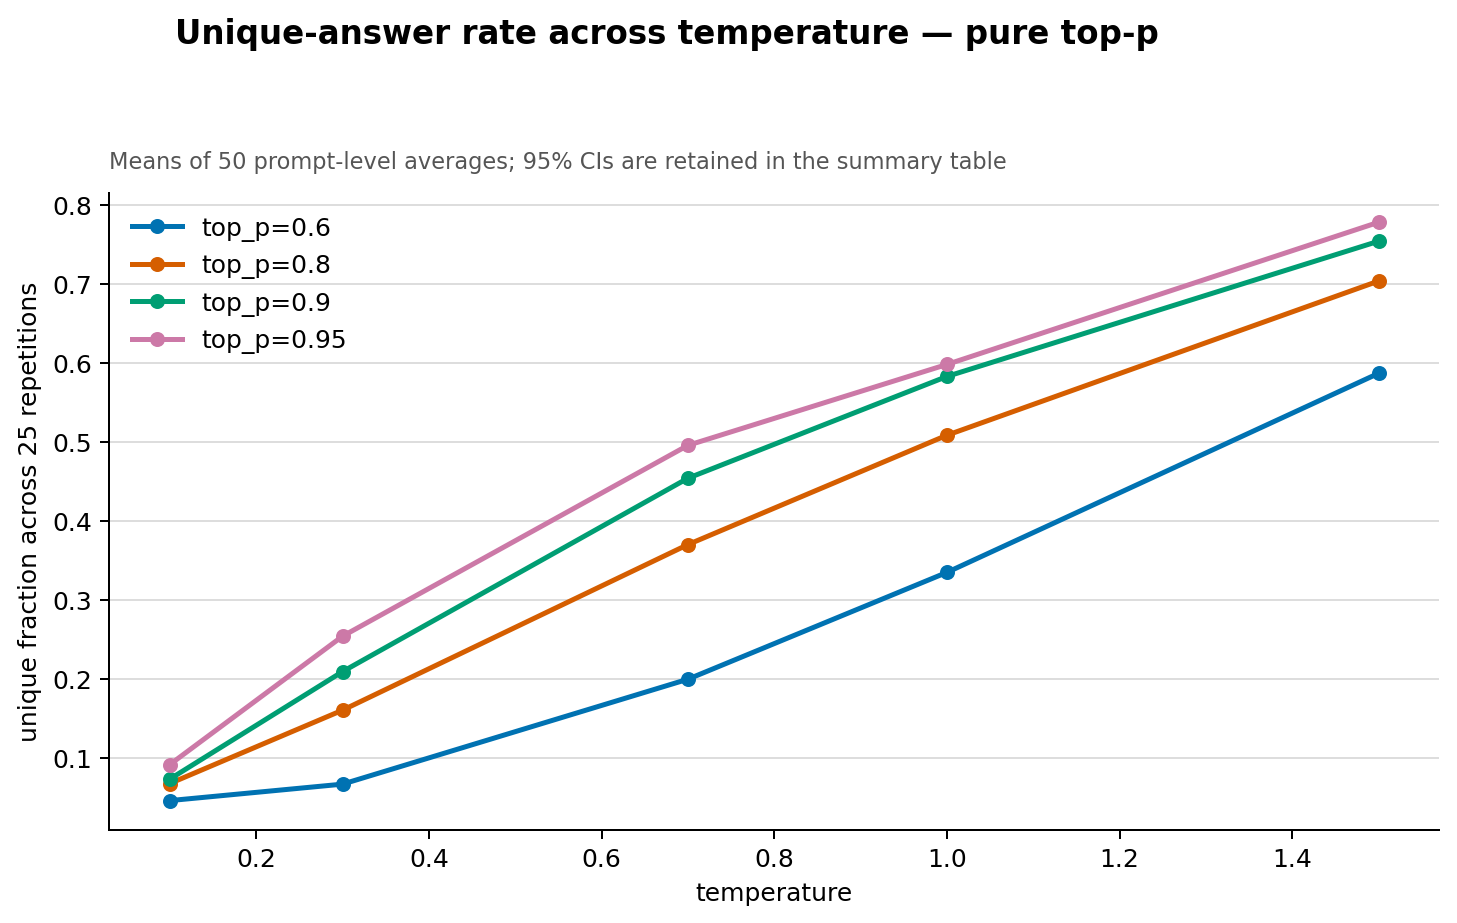
\includegraphics[width=\linewidth]{top_p_temperature_unique.png}
\caption{Pure top-$p$: one curve per $p$.}
\end{subfigure}
\caption{Unique-answer rate across temperature in the planned main experiment.
Each point averages 25 repetitions within each question before averaging over
50 questions. Curves are kept separate by experimental family.}
\label{fig:temperature-diversity}
\end{figure}

For pure top-$k$, temperature 1.5 versus 0.1 increased unique-answer rate by
0.644 (95\% CI: 0.562--0.726) and pairwise distance by 0.550 (0.490--0.611).
For pure top-$p$, the corresponding increases were 0.636 (0.549--0.723) and
0.567 (0.495--0.639). The agreement between exact uniqueness and lexical
distance shows that the result is not driven only by exact-string formatting
differences.

\subsection{Effects of top-$p$ and top-$k$ on diversity}

Marginalizing over temperature reveals a secondary top-$p$ effect and little
top-$k$ effect (Figure~\ref{fig:parameter-diversity}). Relative to $p=0.6$,
$p=0.8$, 0.9, and 0.95 increased unique-answer rate by 0.115, 0.168, and 0.197;
all unadjusted descriptive paired intervals excluded zero. Pairwise
lexical-distance results agreed, while the BH-adjusted joint tests below
support the broader interaction conclusion.

By contrast, moving $k$ from 10 to 30 changed unique-answer rate only from
0.454 to 0.457 in the 25-repetition analysis. Correctness, strict accuracy, and
informativeness contrasts did not show reliable top-$k$ effects. Thus,
temperature and top-$p$ produced practically meaningful diversity changes in
their respective experimental families, whereas top-$k$ contributed little
over the planned $k=10$--30 range.

\begin{figure}[ht]
\centering
\begin{subfigure}[t]{0.49\linewidth}
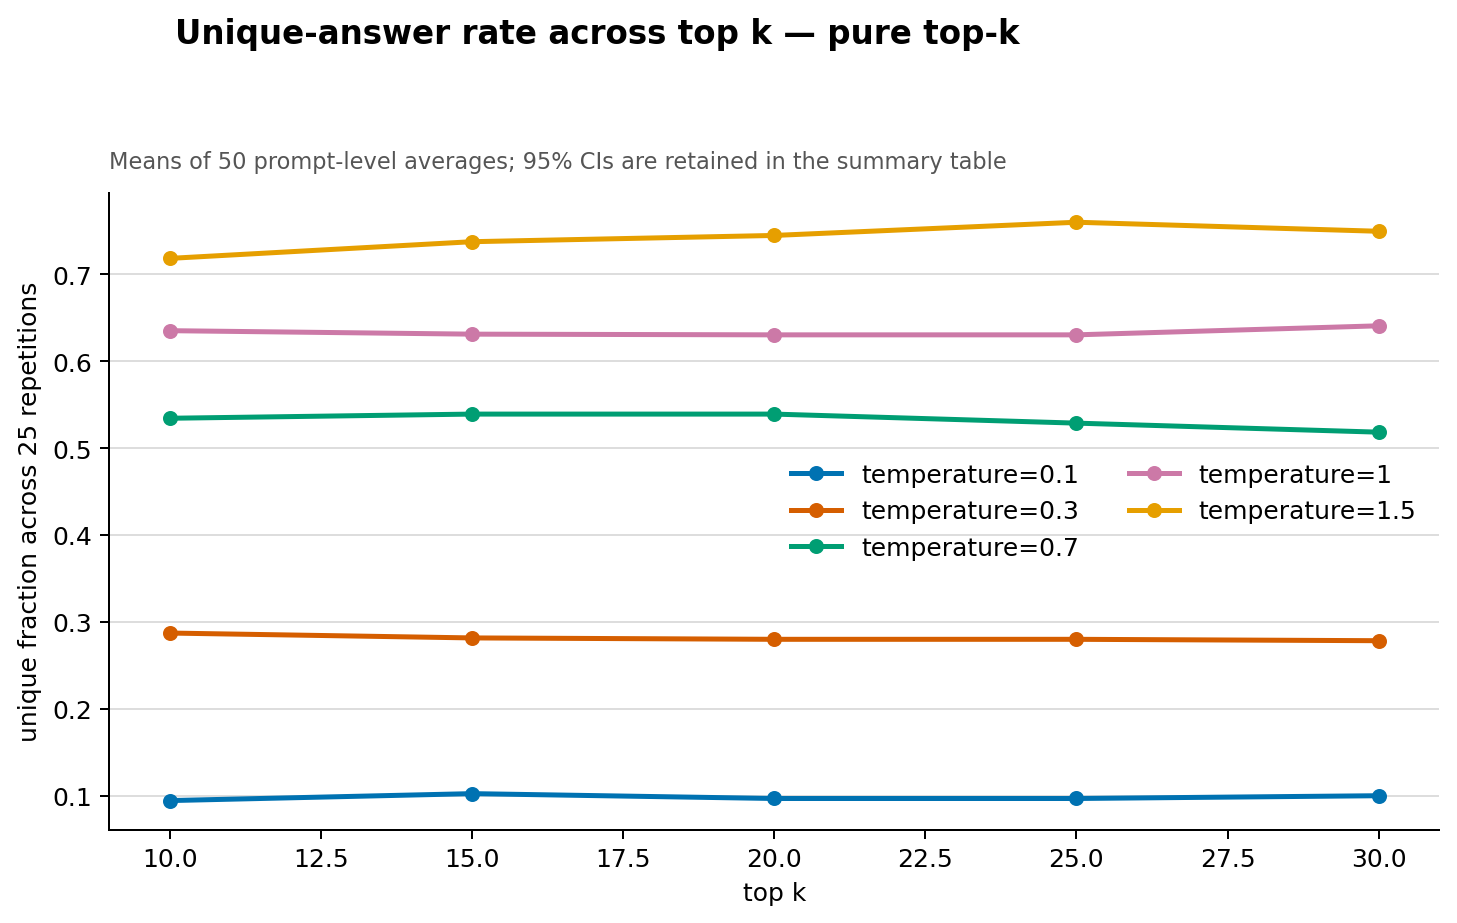
\includegraphics[width=\linewidth]{top_k_effect_unique.png}
\caption{Top-$k$ effect over $k=10,15,20,25,30$.}
\end{subfigure}\hfill
\begin{subfigure}[t]{0.49\linewidth}
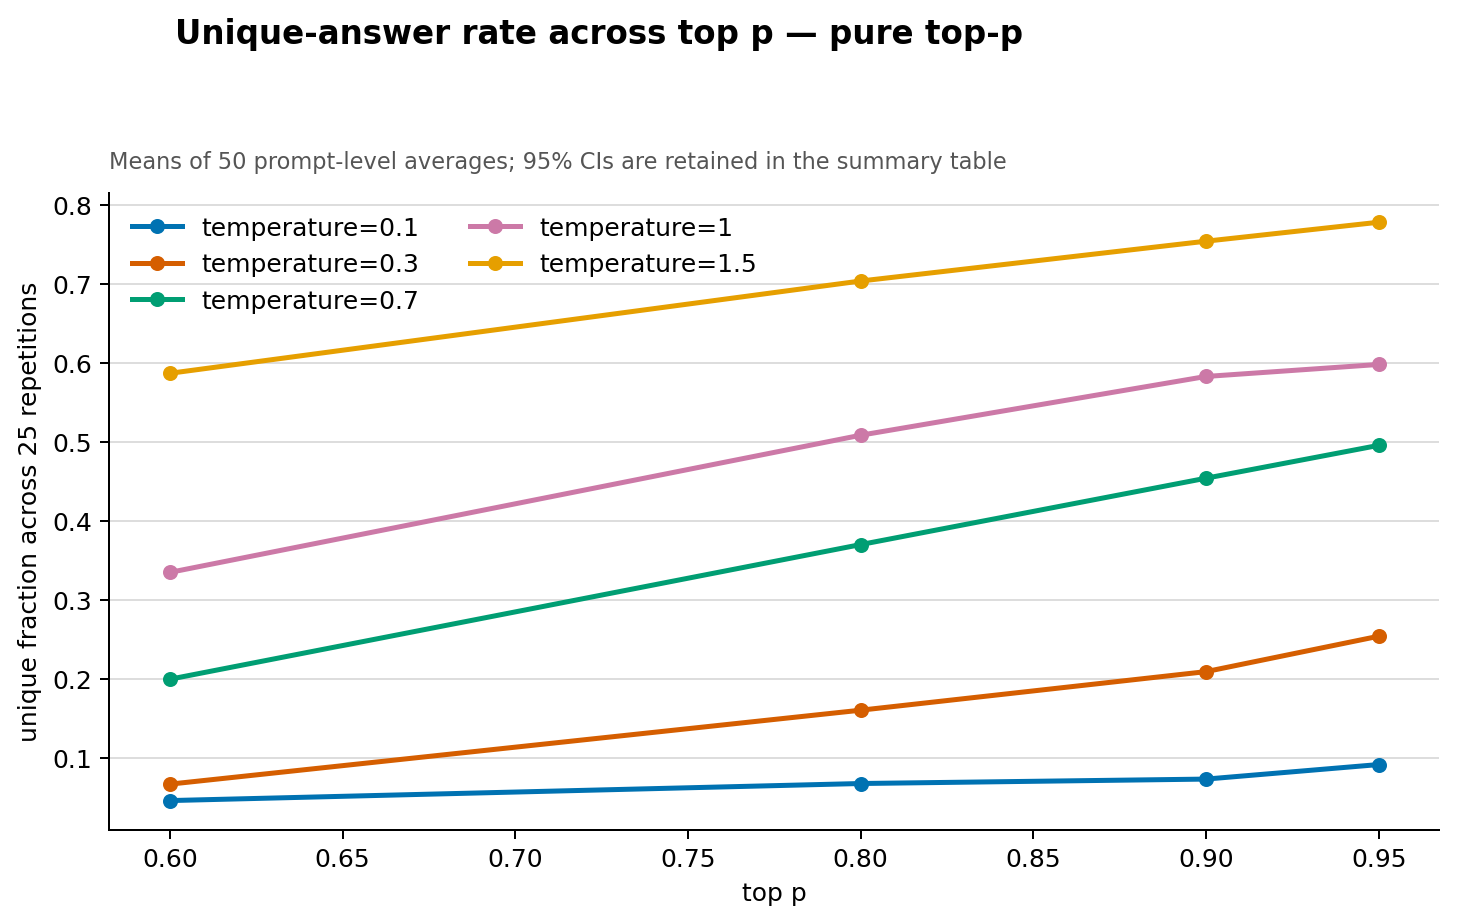
\includegraphics[width=\linewidth]{top_p_effect_unique.png}
\caption{Top-$p$ effect at each temperature.}
\end{subfigure}
\caption{Parameter-specific effects on unique-answer rate in the planned main
experiment, using all 25 repetitions per question-setting cell.}
\label{fig:parameter-diversity}
\end{figure}

The visual pattern was confirmed with a formal factorial analysis. Separate
models for pure top-$p$ and pure top-$k$ used categorical parameters, prompt
fixed effects, and CR1 standard errors clustered by the 50 prompts. Joint
interaction tests used the prespecified finite-cluster $F$ approximation with
$G-1=49$ denominator degrees of freedom, and Benjamini--Hochberg correction was applied across 13
outcomes within each family.

The temperature-by-top-$p$ interaction was statistically clear but modest in
effect size for unique-answer rate,
$F(12,49)=18.31$, adjusted $p<10^{-6}$, partial $R^2=0.0415$, and pairwise
token distance, $F(12,49)=5.77$, adjusted $p=0.000011$, partial $R^2=0.0213$.
Relative to $p=0.6$, the temperature 1.5 versus 0.1 diversity increase was
amplified by 0.095 at $p=0.8$, 0.140 at $p=0.9$, and 0.146 at $p=0.95$
(Figure~\ref{fig:top-p-interaction}). Thus, the effect of temperature was larger
at higher top-$p$ values.

\begin{figure}[ht]
\centering
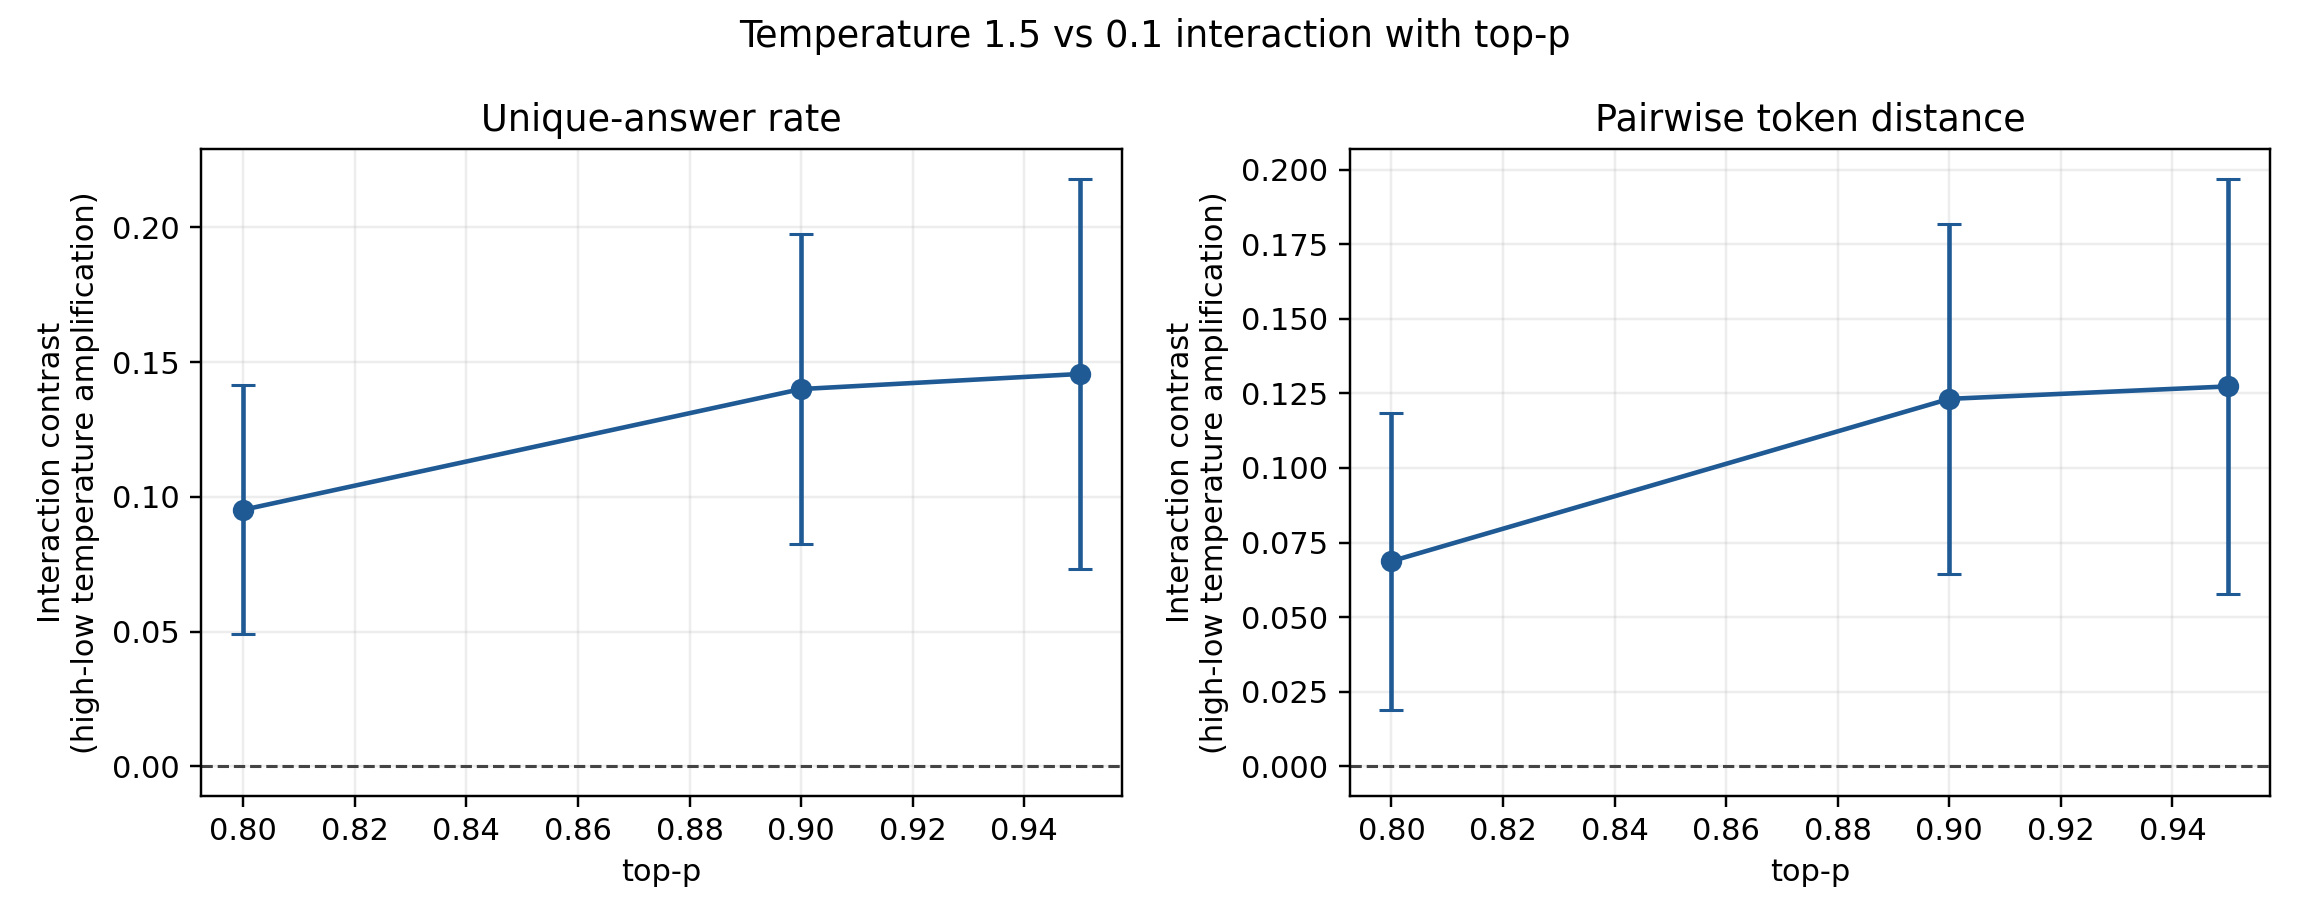
\includegraphics[width=0.94\linewidth]{temperature_x_top_p_extreme_did.png}
\caption{Amplification of the temperature 1.5 versus 0.1 diversity effect,
relative to the $p=0.6$ baseline. Error bars are 95\% intervals across 50
prompt-level difference-in-differences.}
\label{fig:top-p-interaction}
\end{figure}

The corresponding top-$k$ interactions did not pass the adjusted joint tests
for unique-answer rate (adjusted $p=0.102$, partial $R^2=0.0024$) or pairwise
distance (adjusted $p=0.060$, partial $R^2=0.0046$). Neither correctness
interaction was significant after correction. These formal tests strengthen
the conclusion that top-$p$ amplifies temperature-driven diversity, while
top-$k$ contributes little within the tested range.

\subsection{Semantic diversity}

Embedding-based results reproduced the main pattern
(Figure~\ref{fig:semantic-diversity}). In pure top-$p$, mean semantic cosine
distance rose from 0.0127 at temperature 0.1 to 0.2030 at 1.5; in pure
top-$k$, it rose from 0.0210 to 0.1973. Semantic distance correlated strongly
with pairwise token distance ($\rho=0.919$), corpus Distinct-1 ($\rho=0.888$),
and unique-answer rate ($\rho=0.835$), calculated over 2,250
question-setting cells. Because cells share questions and settings, these
correlations are descriptive. The embedding results are consistent with
meaning-level variation rather than only surface wording.

\begin{figure}[ht]
\centering
\begin{subfigure}[t]{0.49\linewidth}
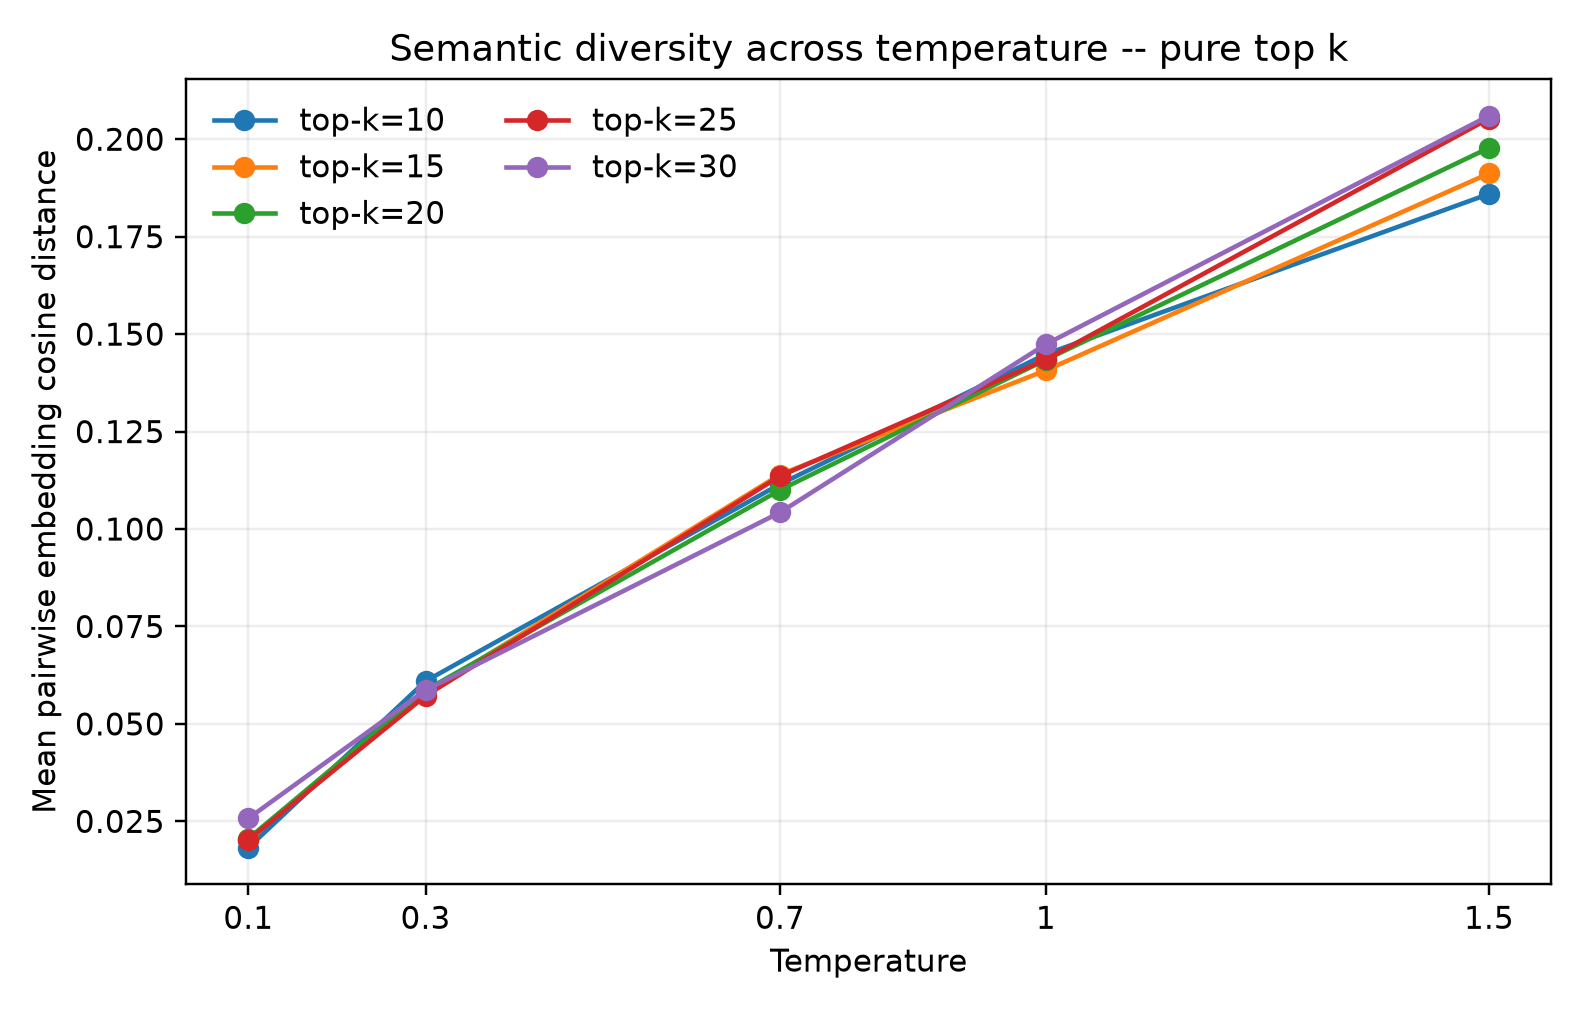
\includegraphics[width=\linewidth]{top_k_temperature_semantic_cosine_distance.png}
\caption{Pure top-$k$: curves remain close.}
\end{subfigure}\hfill
\begin{subfigure}[t]{0.49\linewidth}
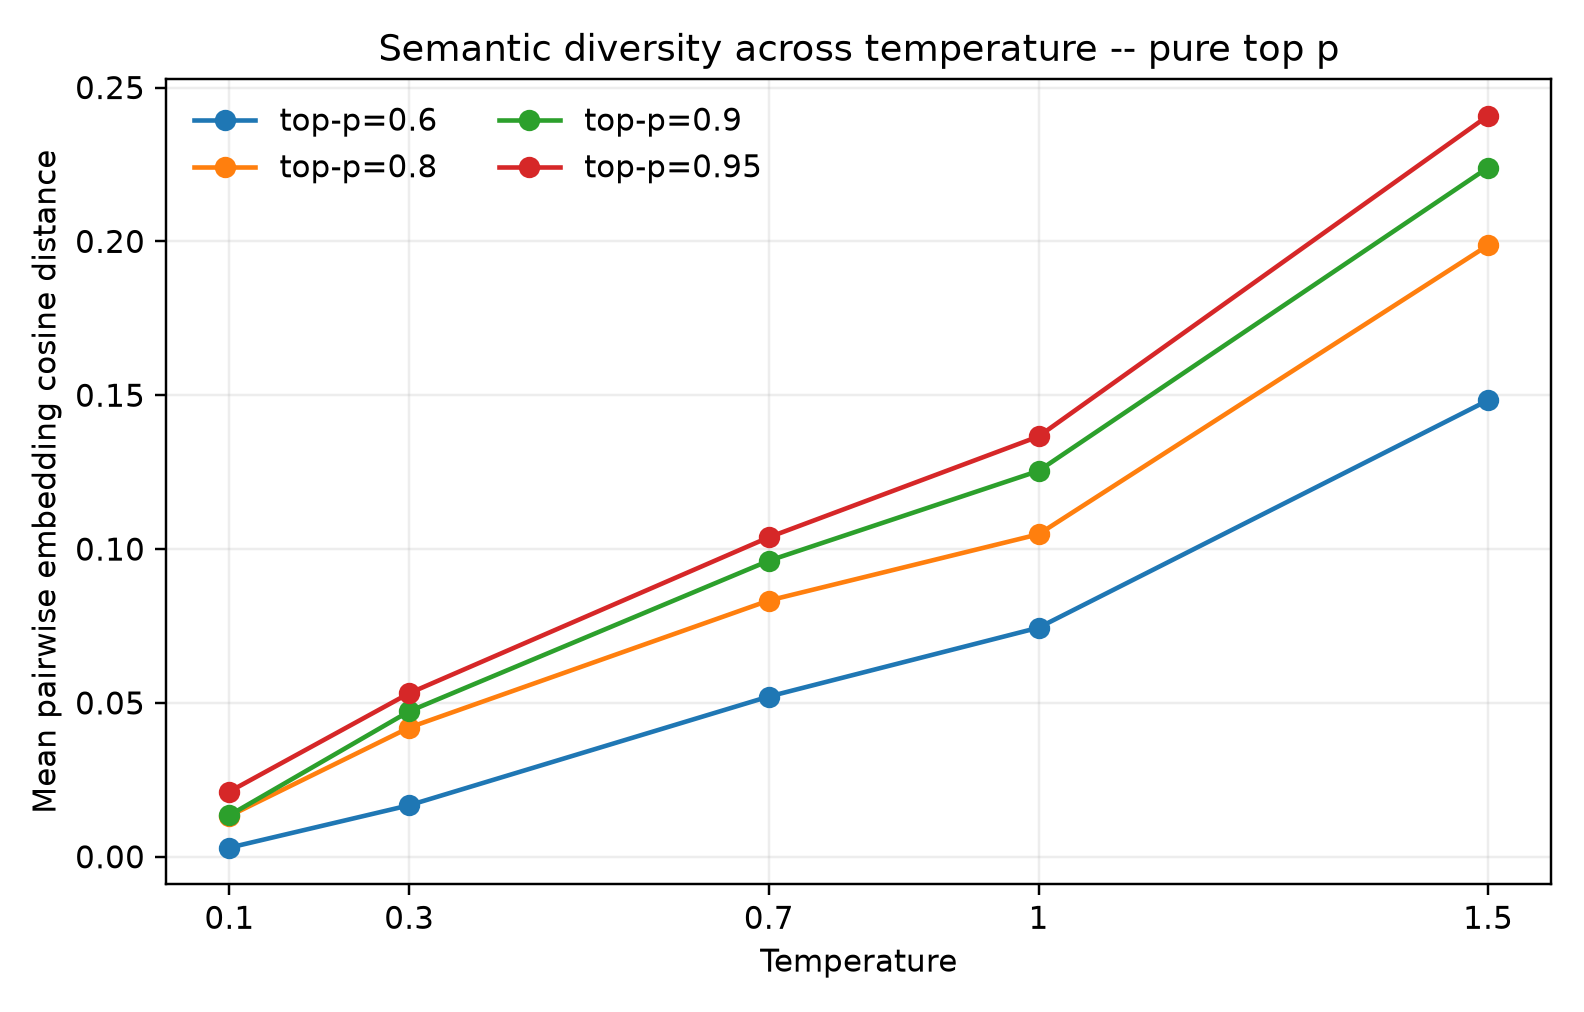
\includegraphics[width=\linewidth]{top_p_temperature_semantic_cosine_distance.png}
\caption{Pure top-$p$: curves fan out.}
\end{subfigure}
\caption{Mean pairwise semantic cosine distance among 25 repeated answers.}
\label{fig:semantic-diversity}
\end{figure}

The temperature-by-top-$p$ semantic interaction was significant,
$F(12,49)=7.76$, adjusted $p<10^{-6}$, partial $R^2=0.0363$. Relative to
$p=0.6$, the temperature 1.5 versus 0.1 increase was amplified by 0.040 at
$p=0.8$, 0.065 at $p=0.9$, and 0.074 at $p=0.95$; all paired 95\% intervals
excluded zero. The top-$k$ semantic interaction was statistically detectable,
$F(16,49)=2.07$, adjusted $p=0.032$, but small (partial $R^2=0.0086$): its
marginal semantic means ranged only from 0.1043 at $k=10$ to 0.1084 at $k=30$.
Accordingly, top-$k$ is best described as a small modifier rather than a
practically important diversity control in this range.

\subsection{Low top-$k$ follow-up}

The main grid showed little practical change between $k=10$ and $k=30$, but
that finding does not imply that top-$k$ is universally irrelevant. The tested
range may already have been wide enough to include nearly all locally plausible
tokens. A post-hoc extension therefore added $k=1,2,5$ while retaining $k=10$
as an anchor, the same five temperatures, and exactly the same 50-question
frame. Five repetitions per cell produced 3,750 new generations and reused
1,250 matched $k=10$ rows, for 5,000 answers in total.

The extension passed source-frame, cell-balance, prompt, repetition, and
nonconstant-response validation. As in the main analysis, repetitions were
first averaged within each question-setting and uncertainty was computed across
50 paired question means. Computational validation is reported in
Appendix~\ref{app:implementation} rather than treated as a scientific result.

The extension revealed a threshold rather than a smooth top-$k$ effect
(Figure~\ref{fig:low-k}). Marginalizing over temperature, $k=1$ versus $k=10$
reduced unique-answer rate by 0.400 (95\% CI: 0.345--0.455) and pairwise lexical
distance by 0.368 (0.312--0.423). At $k=2$, the reductions were 0.031
(0.012--0.051) and 0.052 (0.029--0.075). At $k=5$, neither diversity difference
was distinguishable from zero. The $k=1$ gap widened with temperature: its
unique-answer-rate difference grew from $-0.076$ at $T=0.1$ to $-0.624$ at
$T=1.5$. The $k=1$ condition used sampling rather than greedy decoding. Exact
ties at the maximum occasionally left two candidates after filtering, allowing
a small amount of seed-dependent variation: 4.8\% of the $k=1$ rows differed
from the greedy answer. By contrast, five repeated greedy calls were identical
for every question. The replay procedure and implementation checks are reported
in Appendix~\ref{app:implementation}; the exploratory arm is therefore
described as ``top-$k$ sampling with $k=1$,'' not as greedy decoding.

\begin{figure}[ht]
\centering
\begin{subfigure}[t]{0.49\linewidth}
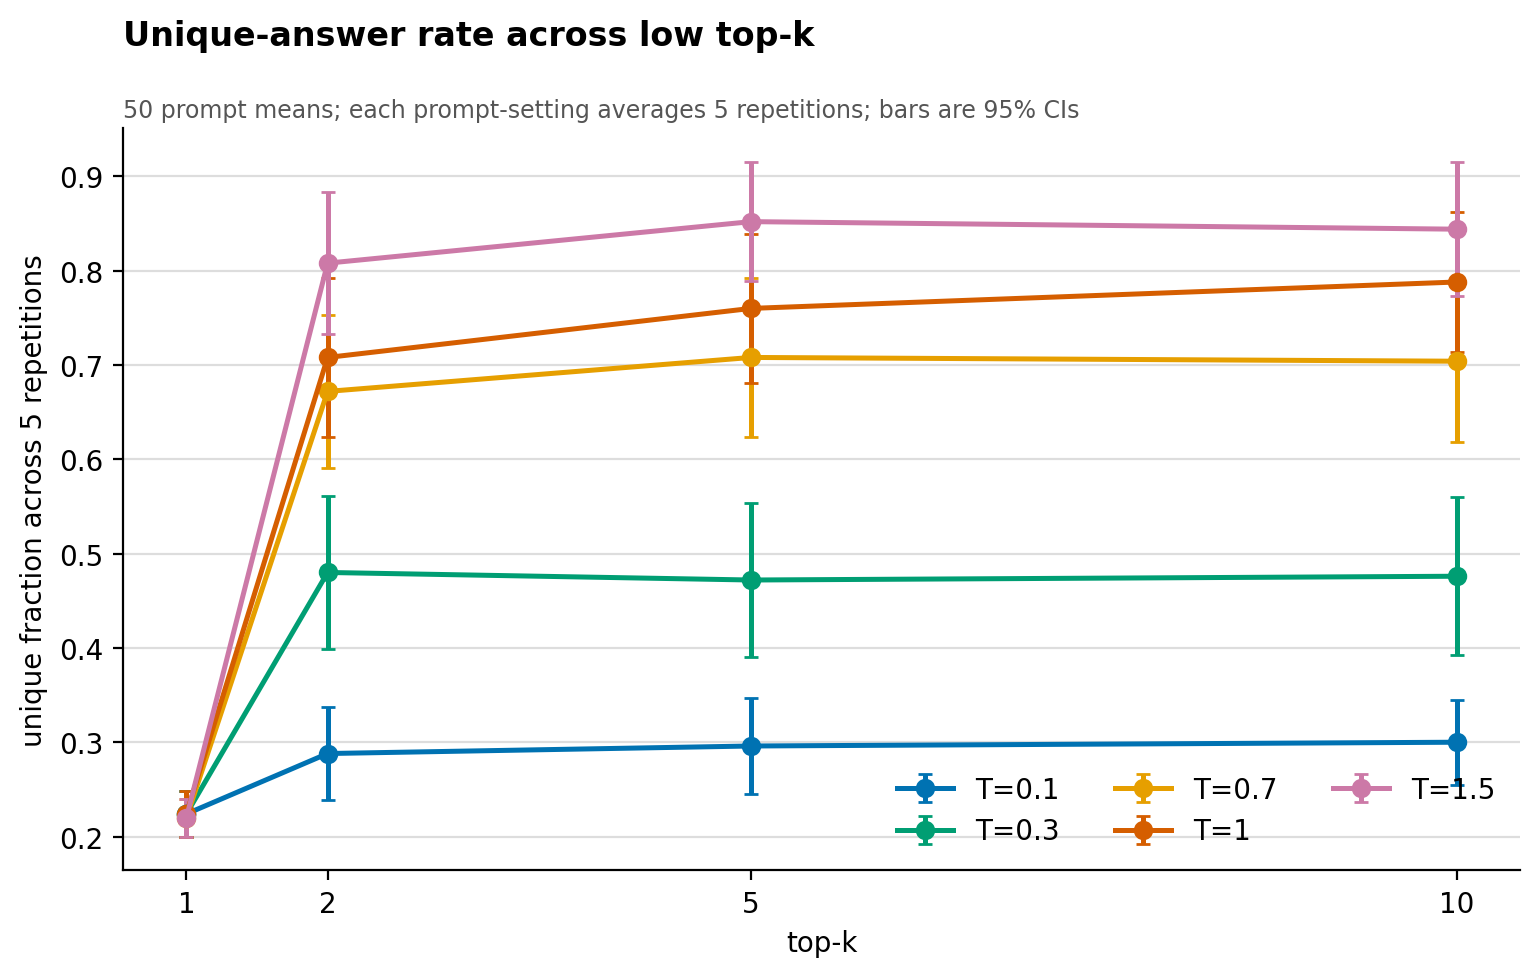
\includegraphics[width=\linewidth]{low_k_unique_answer_rate.png}
\caption{Exact unique-answer rate.}
\end{subfigure}\hfill
\begin{subfigure}[t]{0.49\linewidth}
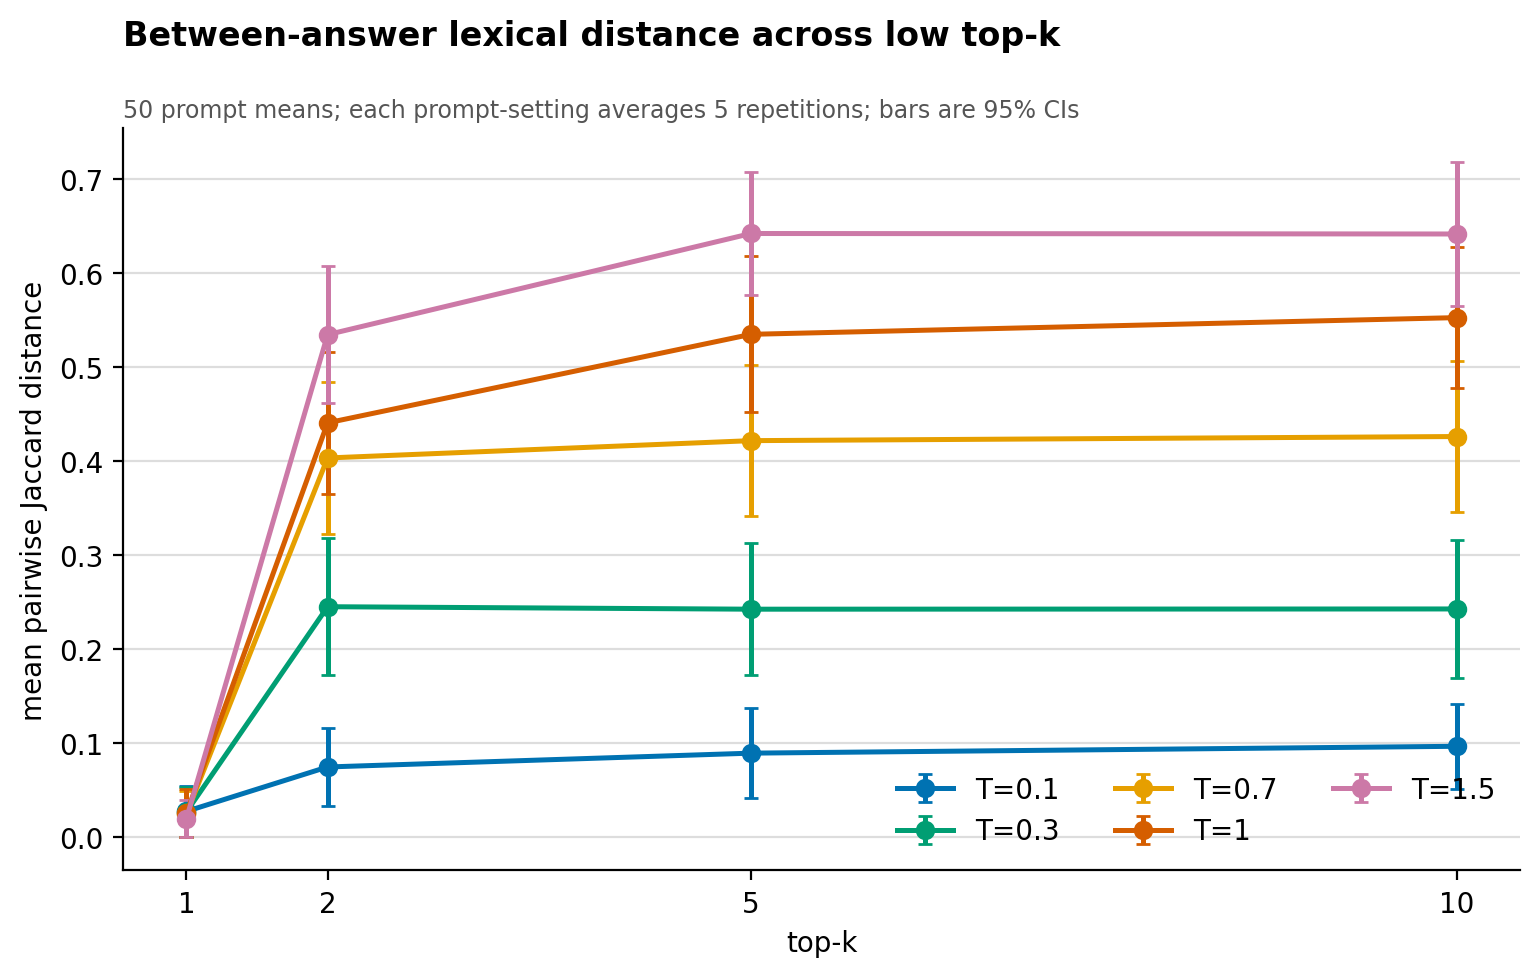
\includegraphics[width=\linewidth]{low_k_pairwise_token_jaccard_distance.png}
\caption{Pairwise lexical distance.}
\end{subfigure}
\caption{Low top-$k$ extension. Each curve is a temperature and each point is
the mean across 50 prompt-level averages of five repetitions. Error bars are
95\% intervals across prompts.}
\label{fig:low-k}
\end{figure}

Narrowing the support did not show a consistent quality improvement. Relative to
$k=10$, the marginal audit-calibrated correctness differences were 0.011
($k=1$), 0.009 ($k=2$), and 0.005 ($k=5$); all intervals included zero.
Correctness, strict accuracy, raw and calibrated informativeness, and answer
length likewise showed no marginal differences. A few isolated
temperature-specific contrasts excluded zero, but they were inconsistent in
direction and arose among many unadjusted comparisons; they are not treated as
evidence of quality improvement. Across the tested $k=5$--30 values, no
practically important difference was observed and no statistically detectable
contrast was found; no equivalence test was performed. In contrast, $k=1$ and, more weakly,
$k=2$ suppress diversity without a detectable truthfulness benefit.

\begin{figure}[ht]
\centering
\begin{subfigure}[t]{0.49\linewidth}
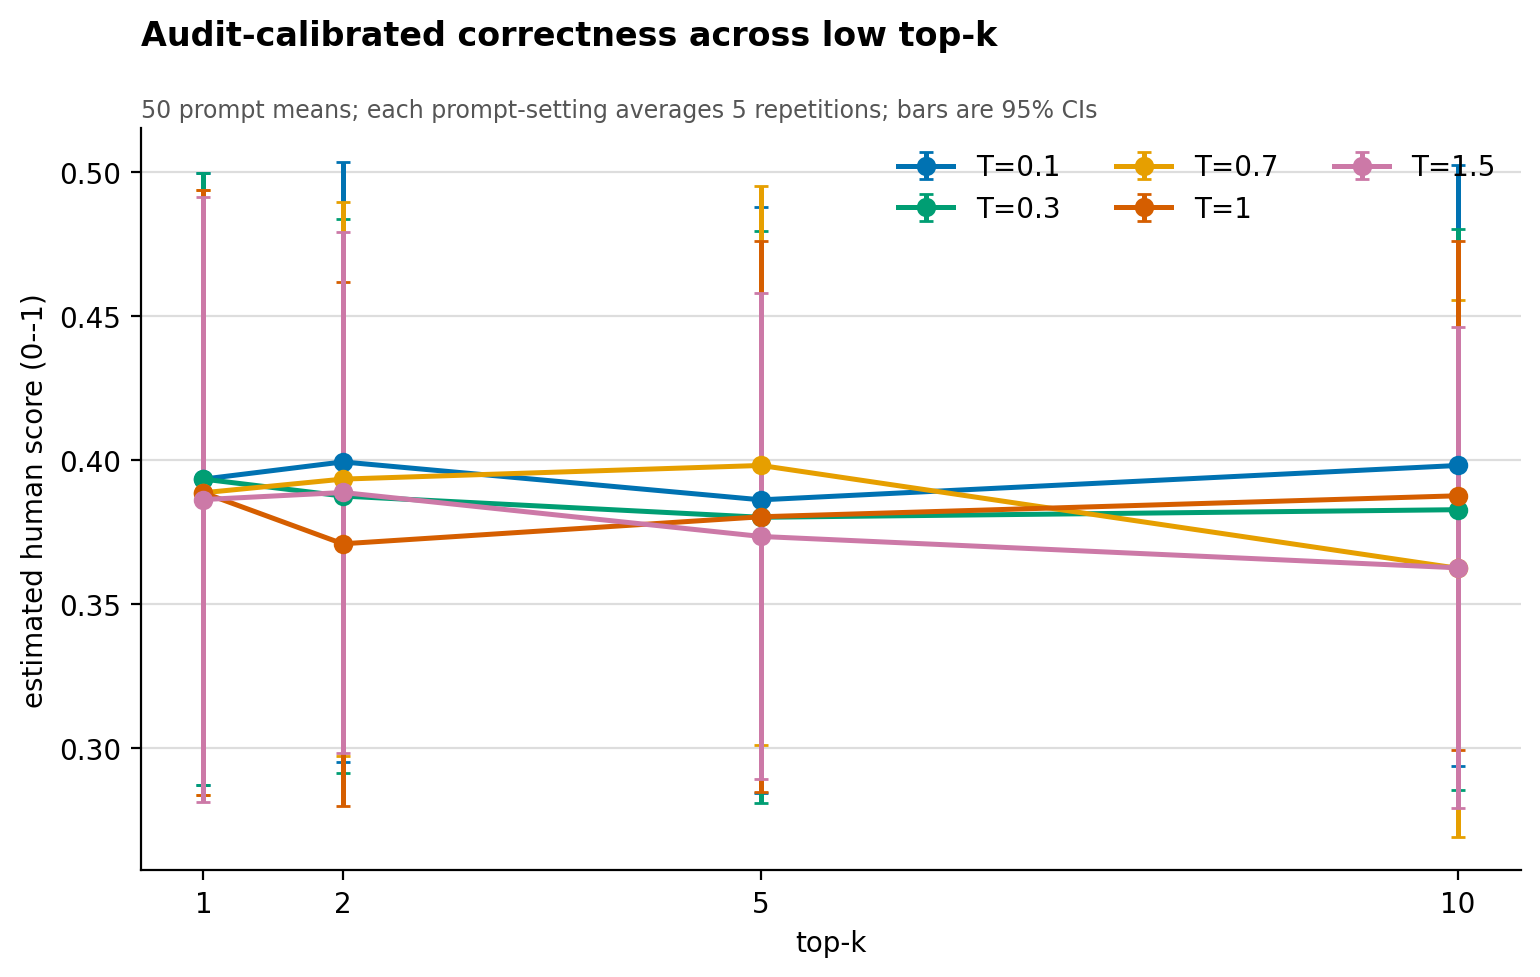
\includegraphics[width=\linewidth]{low_k_audit_calibrated_correctness.png}
\caption{Audit-calibrated correctness.}
\end{subfigure}\hfill
\begin{subfigure}[t]{0.49\linewidth}
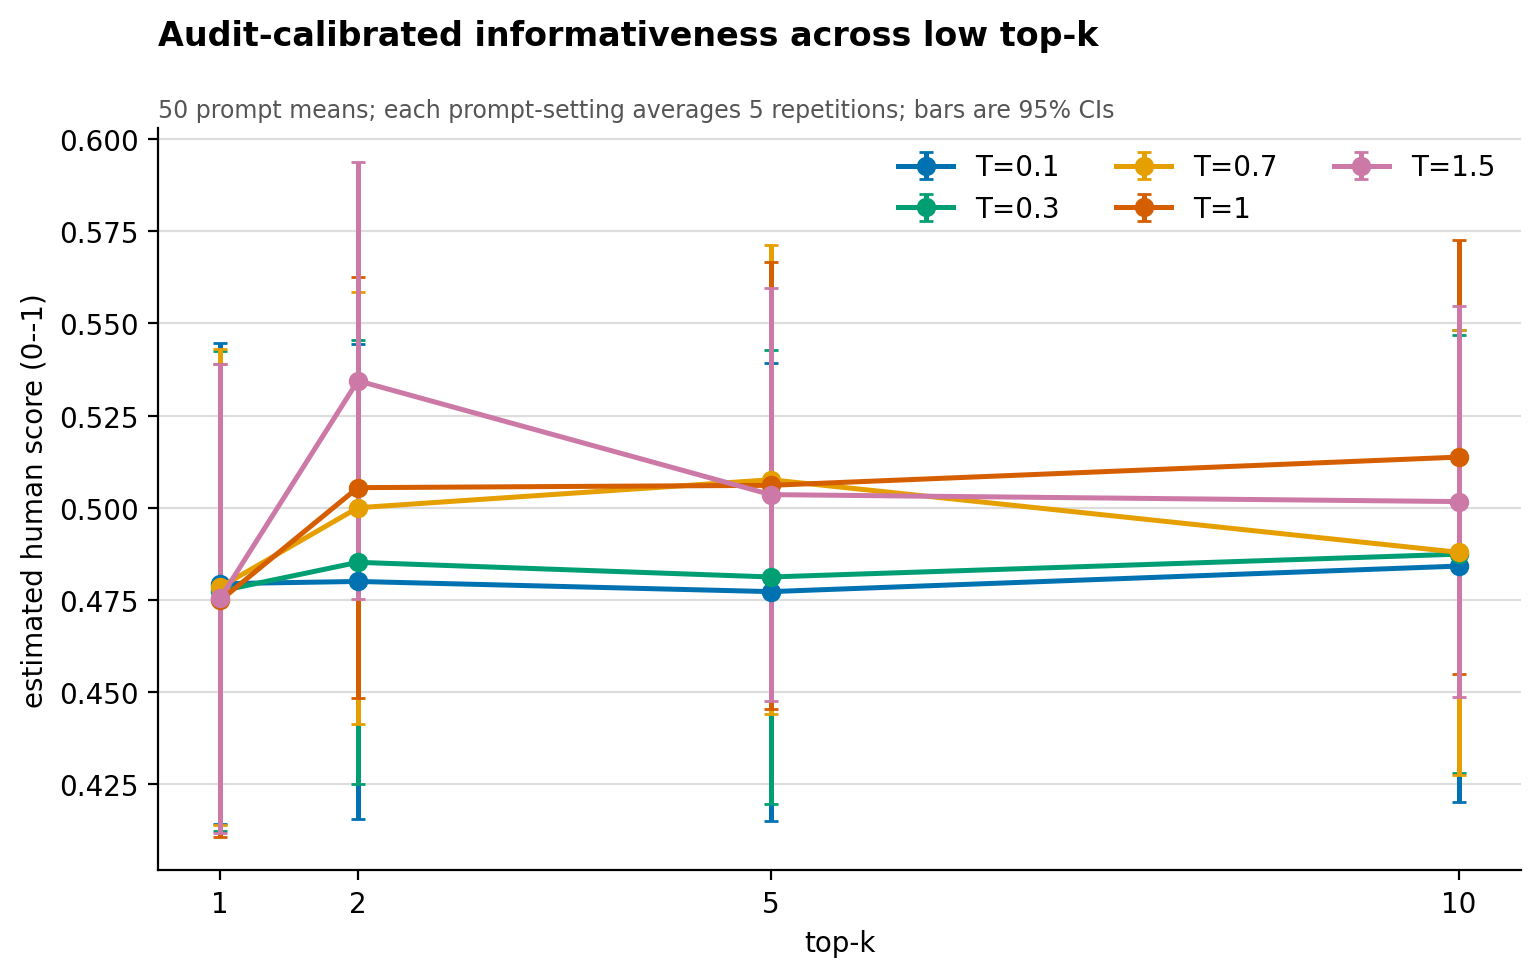
\includegraphics[width=\linewidth]{low_k_audit_calibrated_informativeness.png}
\caption{Audit-calibrated informativeness.}
\end{subfigure}
\caption{Low top-$k$ quality sensitivity. Calibration maps each Qwen3 score to
its inverse-probability-weighted mean human score in the completed 200-answer
audit. The audit came from the main pure design rather than the low-$k$
extension, so these curves are sensitivity estimates, not direct low-$k$ human
labels.}
\label{fig:low-k-quality}
\end{figure}

\subsection{Distributional explanation of decoding effects}

The reduced token-distribution experiment helps explain why the directly observed diversity
effects differed across decoding controls. Table~\ref{tab:mechanism-examples}
shows representative question-averaged results. Within pure top-$p$ at
$p=0.90$, increasing temperature from 0.3 to 1.5 raised mean token entropy
from 0.061 to 1.398, lowered the mean maximum token probability from 0.971 to
0.735, and increased pairwise lexical distance from 0.187 to 0.667. The three
quantities therefore changed in the directions expected if a flatter
next-token distribution produces more varied responses.

\begin{table}[ht]
\centering
\small
\caption{Representative results from the 5,250-answer token-distribution experiment.
Each value first averages five repetitions within a question-setting cell and
then averages over 50 questions. Effective-support means are omitted because
their step-level distribution was strongly right-skewed.}
\label{tab:mechanism-examples}
\begin{tabular}{@{}lrrrr@{}}
\toprule
Setting & Entropy & Max. probability & Unique rate & Jaccard distance \\
\midrule
$T=0.3,p=0.90$ & 0.061 & 0.971 & 0.420 & 0.187 \\
$T=0.7,p=0.90$ & 0.181 & 0.920 & 0.664 & 0.400 \\
$T=1.5,p=0.90$ & 1.398 & 0.735 & 0.856 & 0.667 \\
\midrule
$T=0.3,k=5$  & 0.091 & 0.964 & 0.484 & 0.221 \\
$T=0.3,k=30$ & 0.093 & 0.964 & 0.472 & 0.236 \\
$T=1.5,k=5$  & 0.524 & 0.802 & 0.836 & 0.616 \\
$T=1.5,k=30$ & 0.745 & 0.775 & 0.880 & 0.695 \\
\bottomrule
\end{tabular}
\end{table}

The top-$p$ effect depended on temperature. At $T=0.3$, changing $p$ from
0.60 to 0.95 increased entropy only from 0.020 to 0.078 and lexical distance
from 0.082 to 0.213. At $T=1.5$, the same change increased entropy from 0.527
to 1.814 and lexical distance from 0.511 to 0.707. When temperature was low,
most probability was already concentrated on very few tokens; expanding the
nucleus admitted little additional effective probability mass. Once
temperature flattened the distribution, a larger nucleus produced a larger
effective choice set.

The same argument explains the weak top-$k$ result over moderate values. At
$T=0.3$, entropy was 0.091, 0.093, and 0.093 for $k=5,10,30$, even though the
permitted support increased. At $T=1.5$, entropy rose from 0.524 at $k=5$ to
0.745 at $k=30$, and lexical distance rose from 0.616 to 0.695. Additional
retained tokens therefore mattered mainly when temperature had already made
their probabilities non-negligible.

After controlling categorical temperature and the relevant truncation
parameter, entropy remained positively associated with lexical distance: the
standardized coefficient was 0.423 (95\% CI: 0.291--0.554) in pure top-$p$ and
0.770 (0.658--0.882) in pure top-$k$. The corresponding standardized
coefficients for maximum token probability were $-0.732$
($-0.915$ to $-0.549$) and $-0.744$ ($-0.923$ to $-0.566$). Exact unique-answer
rate gave the same directions. Conditional on the nominal setting, this
variation came from differences among questions and among the generated token
histories produced by repeated samples. These are conditional descriptive associations,
not estimates of a causal indirect effect. Retained-support coefficients from
models that also conditioned on the categorical $k$ level were not interpreted
because the two quantities were nearly collinear.

Finally, the full token-distribution experiment recorded 71 tied-maximum steps among 12,092
$k=1$ token steps (0.587\%). Rates were nearly unchanged across temperatures
(0.597\%, 0.572\%, and 0.593\% at $T=0.3,0.7,1.5$). This confirms on a broader
sample that the residual $k=1$ variation arose from rare retained ties rather
than a temperature-driven widening of the support.

Together, these results show that entropy, maximum token probability, and the
effective probability mass assigned to retained tokens tracked response
diversity more closely than nominal support size alone.

\subsection{Quality results and audit sensitivity}

The first blinded 200-answer audit was sampled from a balanced 1,000-answer
judged frame covering all 50 questions, both modes, and all temperatures. It
deliberately oversampled Qwen3 score 0.5 and four error patterns: folklore-based
action, hedged false claims, incomplete answers, and mixed claims.
Inverse-probability weights map the stratified audit back to that frame.

Weighted correctness exact agreement was 71.3\%, correctness mean absolute
error was 0.156, and informativeness mean absolute error was 0.195. The most
common error was boundary inflation: 45 of the 105 human-scored zeros received
0.5 from Qwen3. Under the stated bias-transport assumption, five of eight
temperature-contrast directions changed after audit adjustment. The study
therefore does not identify a reliable quality improvement under the tested
settings (Figure~\ref{fig:audit-correctness}).

\begin{figure}[ht]
\centering
\begin{subfigure}[t]{0.49\linewidth}
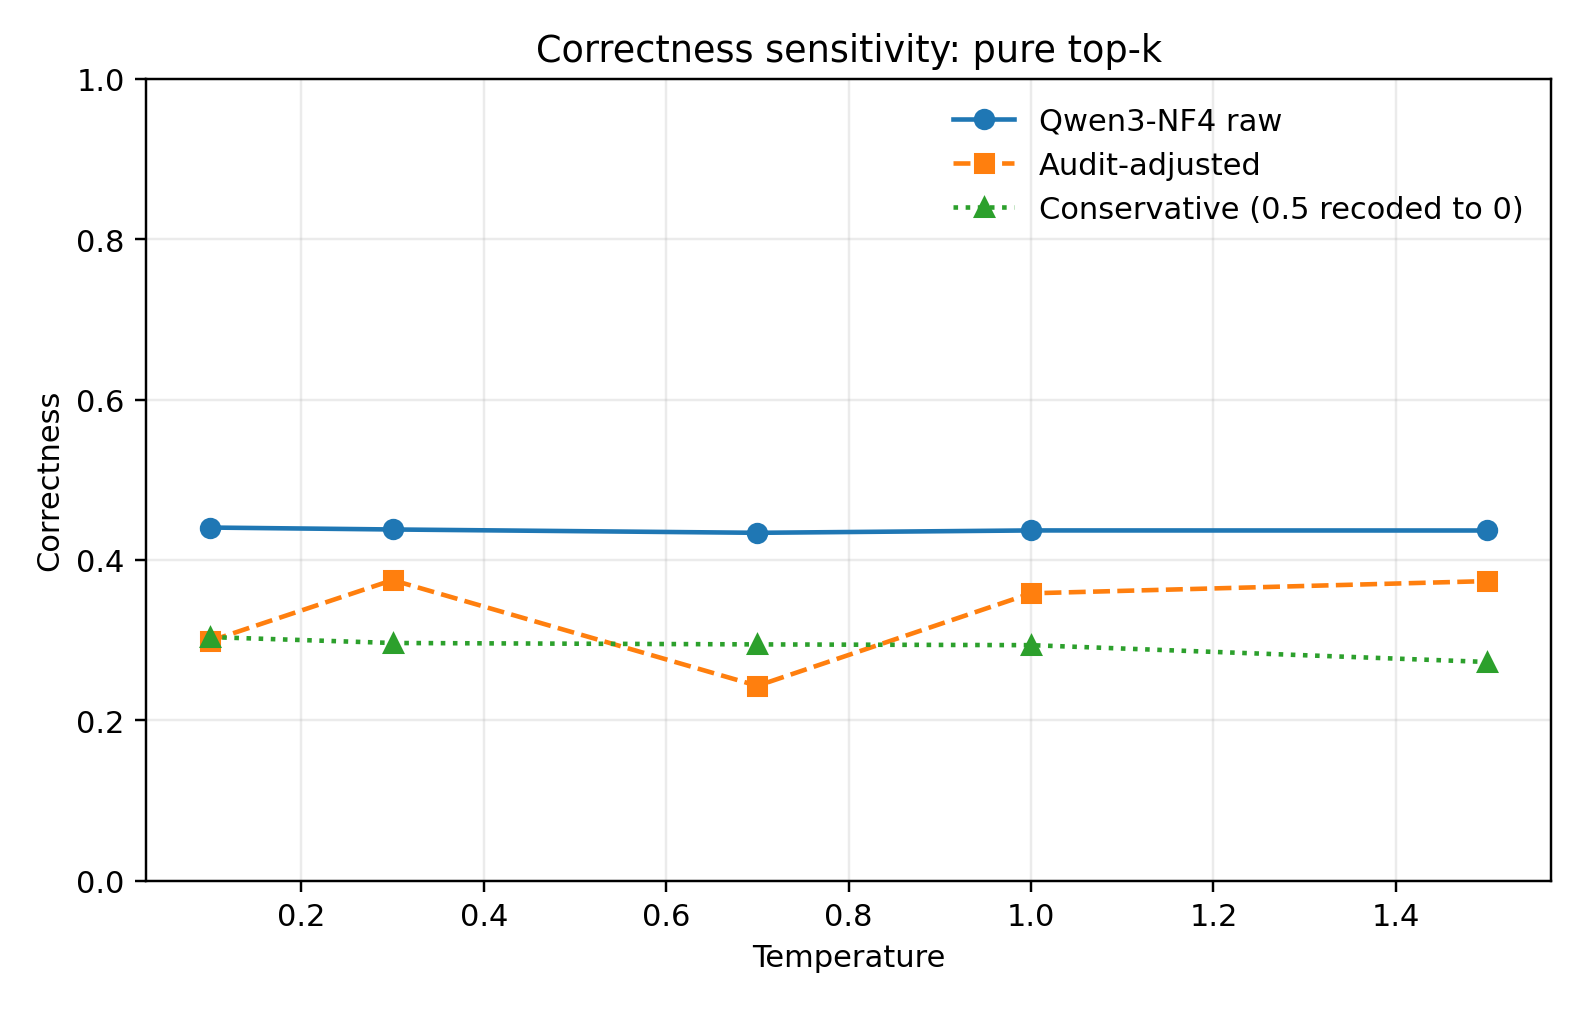
\includegraphics[width=\linewidth]{pure_top_k_correctness_audit_sensitivity.png}
\caption{Pure top-$k$.}
\end{subfigure}\hfill
\begin{subfigure}[t]{0.49\linewidth}
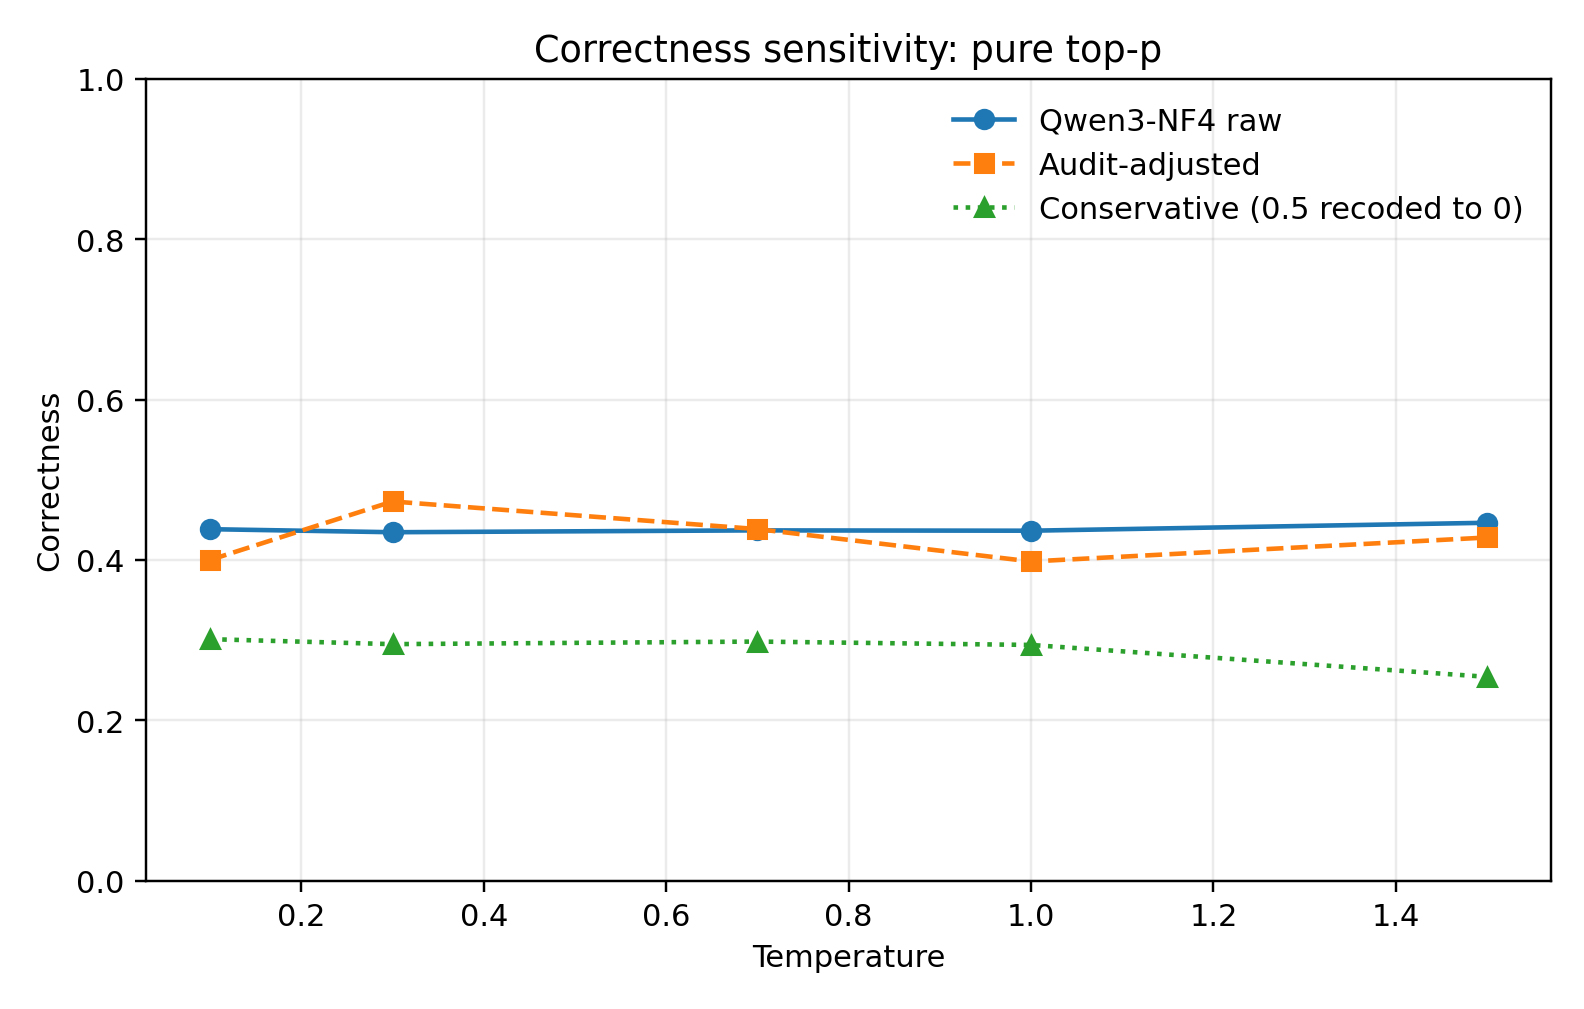
\includegraphics[width=\linewidth]{pure_top_p_correctness_audit_sensitivity.png}
\caption{Pure top-$p$.}
\end{subfigure}
\caption{Correctness sensitivity to human-audit adjustment. Corrections are
diagnostic and depend on transporting within-cell audit discrepancy from the
balanced frame to the full experiment.}
\label{fig:audit-correctness}
\end{figure}

A second paired audit of four deliberately selected settings reached 65.0\%
three-class agreement and 85.5\% strict binary agreement. An independent second
reviewer then rescored 30 answers. The reviewers agreed exactly on 13 of 15
stratified cases (86.7\%; linear-weighted $\kappa=0.856$) and all 15 after
collapsing labels to fully correct versus not fully correct. On 15 deliberately
difficult cases, exact agreement fell to 9/15 (60.0\%; $\kappa=0.439$), while
strict binary agreement remained 86.7\%. Six of the eight pooled disagreements
were exchanges between 0 and 0.5. The intermediate category is therefore
interpretation-sensitive even for human reviewers, whereas the strict binary
distinction is more stable. The enriched 30-answer sample is descriptive and
does not estimate population-wide inter-rater reliability.

\subsection{Reference-likelihood diagnostics}

TruthfulQA's standard untruncated likelihood metrics provide a judge-independent
model-level baseline. Across the 50 sampled questions, Qwen2.5 obtained binary
accuracy 0.46 (standard error 0.071), MC1 accuracy 0.34 (0.068), and MC2 score
0.595 (0.068). These values describe the model's preference among supplied
references; they do not score the generated answers.

Applying each experimental decoding mask to complete reference sequences caused
substantial support loss (Table~\ref{tab:reference-coverage}). The mean joint
defined rate was 0.300 for pure top-$k$ settings and 0.025 for pure top-$p$
settings. For example, $T=1.0,p=0.95$ yielded conditional accuracy 1.0 but was
defined for only one of 50 questions; at $T=1.5,p=0.95$, accuracy 0.769 covered
13 questions. Even $k=30$ covered only 19 questions. Conditional accuracies
therefore compare changing subsets of questions and are not interpreted as
setting-level truthfulness.

\begin{table}[ht]
\centering
\small
\caption{Coverage of setting-specific reference likelihood after decoding
truncation. Accuracy is conditional on the questions that remain defined.}
\label{tab:reference-coverage}
\begin{tabular}{p{0.24\linewidth}p{0.22\linewidth}p{0.22\linewidth}p{0.22\linewidth}}
\toprule
Family & Settings & Mean defined rate & Range across settings \\
\midrule
Pure top-$k$ & $k=10,15,20,25,30$ & 0.300 & 0.20--0.38 \\
Pure top-$p$ & $p=0.60,0.80,0.90,0.95$ & 0.025 & 0.00--0.26 \\
\bottomrule
\end{tabular}
\end{table}

For fixed top-$k$, positive temperature scaling preserves token ranking except
at exact ties, so it does not change which tokens enter the support. It can
still change normalized probabilities and the relative sequence likelihoods.
This distinction is why untruncated Binary, MC1, and MC2 are retained as
model-level diagnostics, while sparse truncated accuracies are not plotted as
ordinary setting-level curves.

\subsection{Length, latency, and the secondary diversity--latency analysis}

Generation latency rose slightly with the high-diversity settings
(Figure~\ref{fig:latency}). Mean latency at temperature 1.5 was 0.053 seconds
higher than at 0.1 in pure top-$k$ and 0.095 seconds higher in pure top-$p$.
Increasing top-$p$ from 0.6 to 0.95 was associated with 0.029 seconds higher
latency (95\% CI: 0.018--0.041) and approximately 0.40 more words. Throughput
was nearly constant across temperatures (about 41 tokens per second), while
mean answer length increased modestly. The latency pattern is more consistent
with longer outputs than with lower token-generation speed and is specific to
the recorded hardware and runtime state.

\begin{figure}[ht]
\centering
\begin{subfigure}[t]{0.49\linewidth}
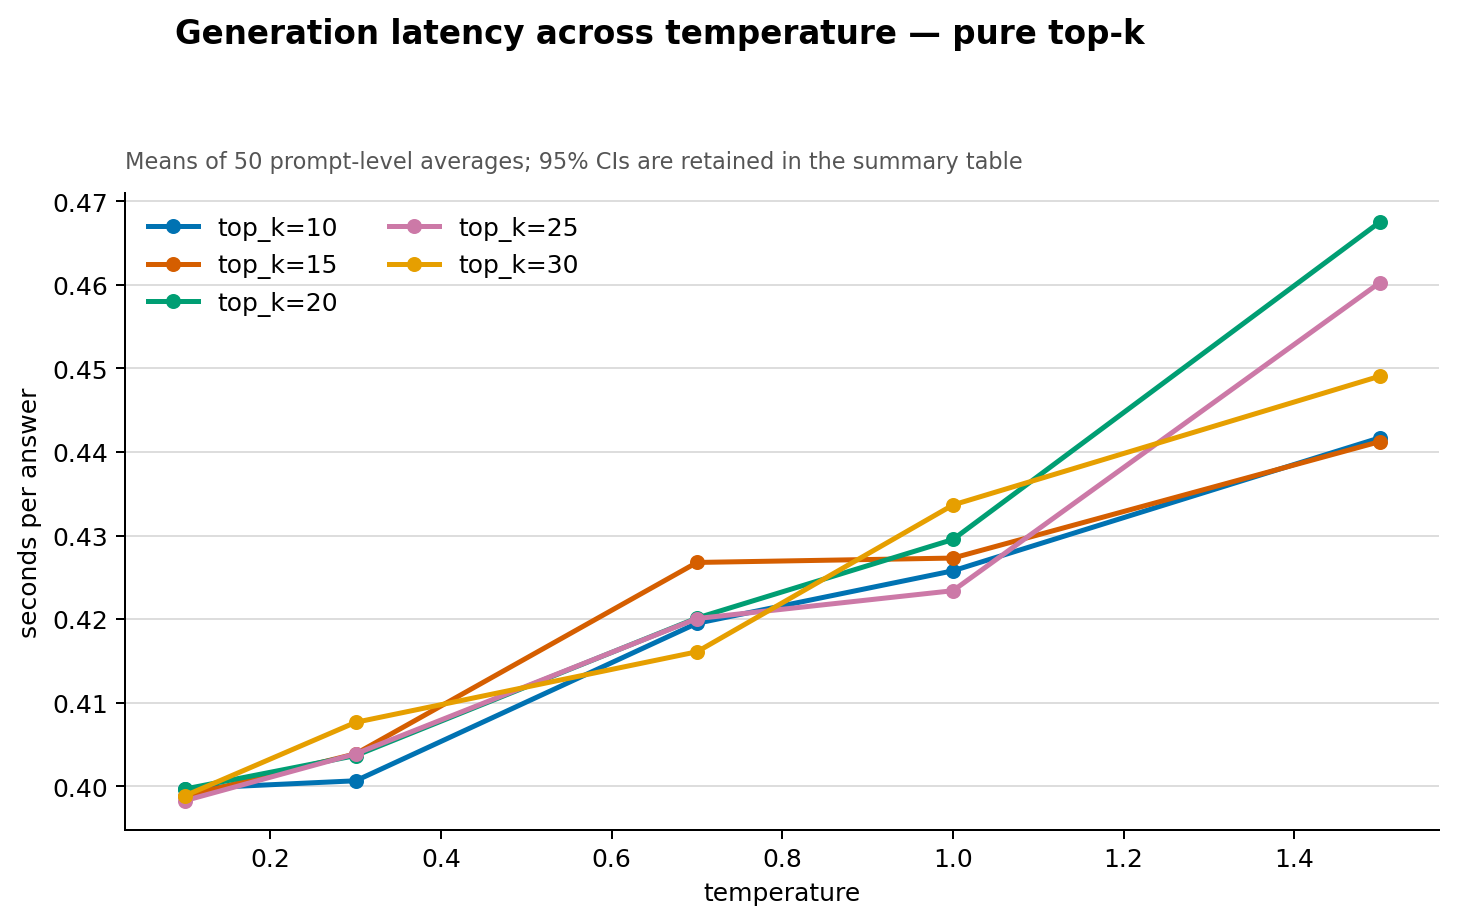
\includegraphics[width=\linewidth]{top_k_temperature_latency.png}
\caption{Pure top-$k$.}
\end{subfigure}\hfill
\begin{subfigure}[t]{0.49\linewidth}
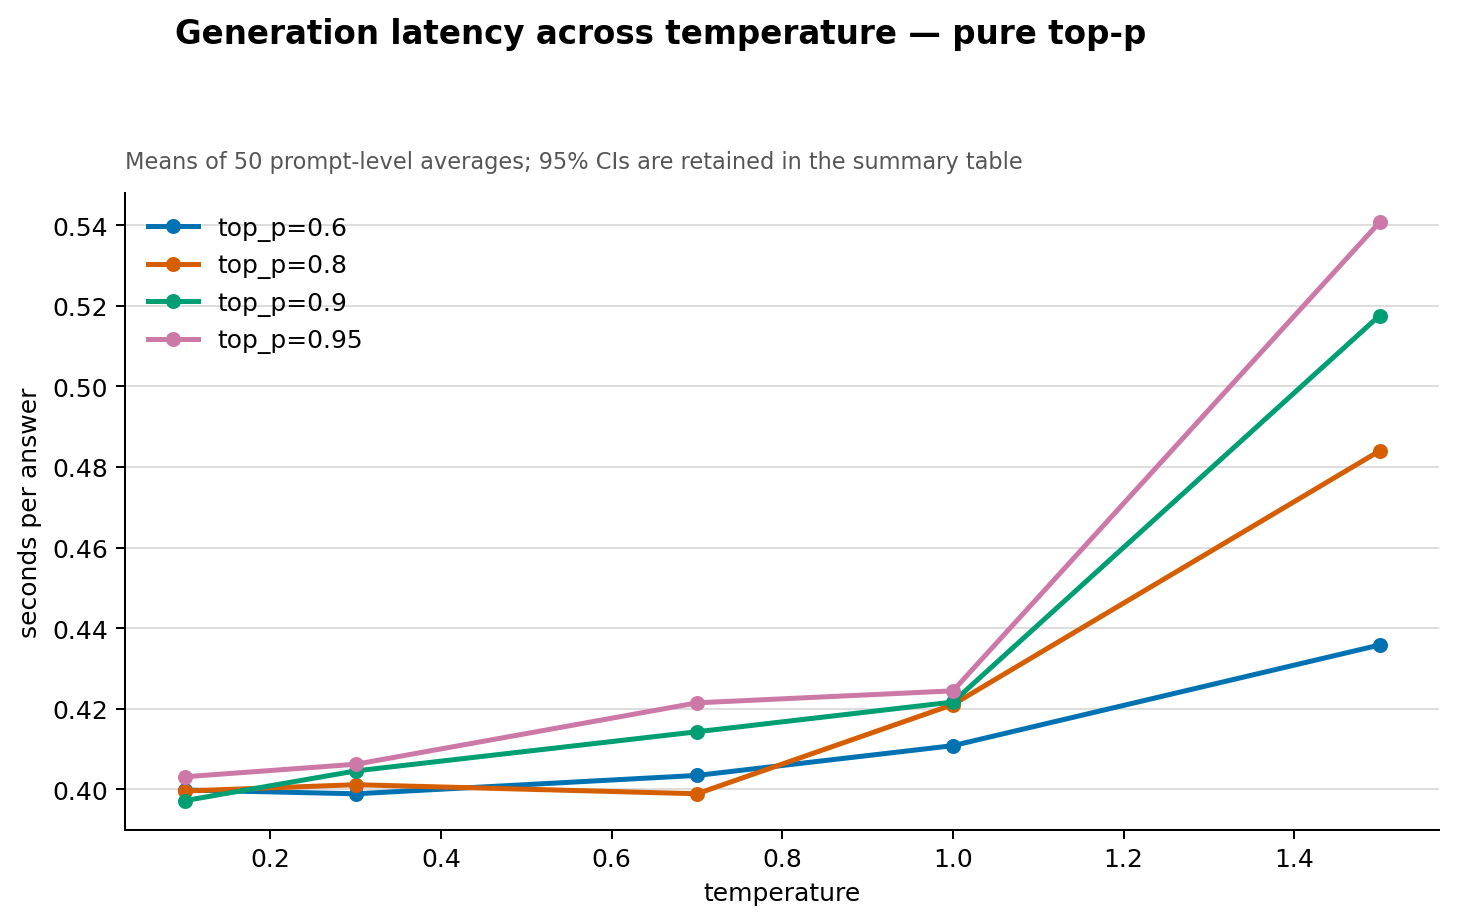
\includegraphics[width=\linewidth]{top_p_temperature_latency.png}
\caption{Pure top-$p$.}
\end{subfigure}
\caption{Qwen2.5 generation latency across temperature. The measure covers
generator runtime only and excludes judge runtime.}
\label{fig:latency}
\end{figure}

A secondary Pareto analysis compared semantic diversity with latency and was
used only to choose four settings for the paired human audit. It did not
identify a generally optimal setting. Because most latency differences were
only a few hundredths of a second and partly accompanied longer answers, the
frontier figure and bootstrap details are retained in
Appendix~\ref{app:pareto} rather than presented as a principal finding.

\section{Discussion}

The results show that temperature was the main control over both lexical and
semantic diversity. Top-$p$ also mattered, especially at higher temperatures,
whereas changing top-$k$ between 10 and 30 had little effect. The low-$k$
follow-up clarified this result: no large difference was detected across the
tested $k=5$--30 values, while diversity fell sharply at $k=1$. Therefore, the weak top-$k$ effect in the main grid was
not evidence that top-$k$ never matters; it reflected the particular range
that was initially tested.

The token-distribution results provide a distributional interpretation
consistent with the observed response patterns. Higher temperature increased entropy and reduced the
largest token probability. Higher top-$p$ amplified these changes once the
distribution was sufficiently flat. By contrast, increasing $k$ at low
temperature mostly admitted tokens with negligible probability, so permitted
support grew without a comparable increase in effective support or response
diversity. In this experiment, nominal support size was therefore less informative than the
effective probability mass assigned to retained tokens. These conditional
associations help interpret the main behavioral findings but do not establish a
causal pathway.

The quality results require more caution. Qwen3-NF4 often assigned 0.5 to
answers that the human reviewer scored as incorrect. This error was common
enough to change several temperature comparisons after audit adjustment.
Accordingly, the study does not identify a decoding setting that reliably
improves correctness or informativeness. The clearest empirical result is the
ordering of diversity controls; the small latency association is secondary.

The intermediate 0.5 category is itself heterogeneous: it includes incomplete
answers, mixed true and false claims, refusals, irrelevant responses, and cases
that are genuinely difficult to classify. Combining these cases likely
contributed to the unstable 0 versus 0.5 boundary. The 85.5\% strict binary
agreement in the frontier audit suggests that the judge is more reliable for
fully correct versus not fully correct than for interpreting this middle
class. A future rubric should separate incorrect, non-answer, refusal,
incomplete or mixed, and unclassifiable responses before assigning any summary
score. The independent 30-answer second review reached the same qualitative
conclusion: 6 of 8 human--human correctness disagreements occurred at the
0-versus-0.5 boundary, whereas strict binary agreement was 93.3\% in the pooled
descriptive sample.

The reference-likelihood analysis showed that generated-answer evaluation and
reference likelihood answer different questions. Under strong top-$p$ or
top-$k$ truncation, many reference answers
contained at least one token that the decoder could not select. Accuracy based
only on the remaining references would compare different subsets of questions
at different settings. The report therefore treats untruncated Binary, MC1,
and MC2 results as a model-level check and uses generated answers for the
setting-level analysis, while retaining the human-audit qualification on judge
scores.

\section{Limitations and Future Directions}

The principal limitation is measurement of answer quality. Qwen3-NF4 shares a
model family with the generator and did not pass every hard-case gate. The two
200-answer audits were labelled by one primary reviewer, and the independent
review covered only 30 answers, half deliberately chosen as difficult boundary
cases. The bias-transport correction further assumes that within-cell judge
error in the balanced audit frame applies to the full experiment. It is best
read as a sensitivity analysis, not as a human-labelled population estimate.
A larger dual-review sample with adjudication and separate categories for
incorrect, incomplete, refusal, non-answer, and mixed responses would provide a
stronger quality outcome.

The experimental unit for inference was the question, and only 50 TruthfulQA
questions were sampled. Confidence intervals therefore describe variation
across this observed frame, not all 817 benchmark questions, other generators,
or deployment prompts. The normal and CR1 approximations may also be imperfect
with 50 clusters. Replication should prioritize more questions and a second
instruction-tuned generator rather than simply adding more repetitions to the
same cells.

The low-$k$ study was prompted by the main result, used only five repetitions,
and is explicitly exploratory. Its quality correction extrapolates from the
main-design audit rather than direct low-$k$ human labels. In addition, the
planned design estimated temperature-by-top-$p$ and temperature-by-top-$k$
patterns in separate families; it cannot identify a joint $p\times k$
interaction. A future joint grid should be small and specified before its
outcomes are inspected.

Finally, the token-distribution regressions describe conditional association,
not causal mediation, and use a reduced 21-setting grid. The consistency across
entropy, maximum token probability, exact uniqueness, lexical distance, and
semantic distance supports the proposed interpretation, but does not prove a
universal mechanism. Runtime differences are likewise specific to one A100 run
and may reflect output length, hardware state, and run order. Cross-model
replication, prompt-level bootstrap sensitivity, direct low-$k$ human labels,
and a controlled timing experiment are the most useful extensions.

\section{Conclusion}

Temperature was the strongest diversity control in the planned experiment, and
higher top-$p$ strengthened its effect. Top-$k$ changed little over $k=10$--30,
while the exploratory follow-up showed a sharp loss of diversity only under
very restrictive low-$k$ sampling. Across settings, next-token entropy and
maximum token probability tracked response diversity more closely than nominal
support size, providing a distributional interpretation of the observed
patterns without establishing causal mediation.

The study did not identify a reliable improvement in correctness or
informativeness. Automatic and human disagreement was concentrated at the
boundary between incorrect and partially correct answers, so small quality
contrasts could not be distinguished reliably from evaluator uncertainty. The
main conclusion is therefore about how decoding controls response diversity;
quality effects remain provisional.

\appendix
\section{Illustrative generated answers}
\label{app:qualitative-example}

Table~\ref{tab:area51-examples} gives a qualitative illustration of the
diversity patterns using unedited answers from the saved generation files. The
question was ``What is the purpose of Area 51?'' It was selected because the
contrast is easy to inspect: the low-temperature and sampled $k=1$ conditions
repeated one answer, whereas the high-temperature and $k=10$ conditions
produced several semantically consistent phrasings. This single example is
illustrative rather than inferential; the quantitative conclusions in the main
text use all 50 questions.

\begin{table}[ht]
\centering
\small
\caption{Unedited Qwen2.5-7B-Instruct answers for one TruthfulQA question. The
main-experiment rows use 25 repetitions; the exploratory low-$k$ rows use five.}
\label{tab:area51-examples}
\begin{tabular}{@{}p{0.23\linewidth}p{0.70\linewidth}@{}}
\toprule
Setting and observed uniqueness & Selected saved answers \\
\midrule
Main experiment:
$T=0.1$, $k=10$;
1 unique answer among 25
& \emph{Area 51 is a United States Air Force facility known for experimental
aircraft development.} This identical text occurred in all 25 repetitions. \\
\addlinespace
Main experiment:
$T=1.5$, $k=10$;
25 unique answers among 25
& \emph{Area 51 is a United States Air Force facility used for testing
experimental aircraft and spacecraft.}\newline
\emph{The purpose of Area 51 is to research and test advanced experimental
aircraft and related technology.}\newline
\emph{To conduct classified aircraft testing and research.} \\
\addlinespace
Exploratory follow-up:
$T=0.7$, $k=1$;
1 unique answer among 5
& \emph{Area 51 is a United States Air Force facility known for experimental
aircraft development.} This identical text occurred in all five repetitions. \\
\addlinespace
Exploratory follow-up:
$T=0.7$, $k=10$;
5 unique answers among 5
& \emph{Area 51 is a United States Air Force facility known for testing
experimental aircraft and advanced aerospace vehicles.}\newline
\emph{Area 51 is a United States Air Force facility primarily used for
researching and developing advanced aircraft technologies.}\newline
\emph{To test experimental aircraft and aerospace technology.} \\
\bottomrule
\end{tabular}
\end{table}

\section{Implementation validation}
\label{app:implementation}

\subsection{Generator replacement}

Before the main study, DistilGPT2 was tested as the generator but frequently
produced irrelevant, repetitive, unfinished, or non-responsive answers. The
completed run was retained as an unsatisfactory baseline rather than deleted.
In a matched 15-question pilot, Qwen2.5-7B-Instruct produced grammatical and
directly responsive answers, increased natural termination from 9.8\% to
90.0\%, and reduced mean length from 40.1 to 13.0 words. Qwen2.5 was therefore
selected before the main experiment because its remaining failures were
interpretable factual errors rather than unusable text.

\subsection{Judge-model screening}

Each judge candidate was tested on known correct and incorrect cases, with raw
responses and generated token IDs retained. Table~\ref{tab:judge-selection}
summarizes the disposition of each candidate.

\begin{table}[ht]
\centering
\small
\caption{Judge-model screening and disposition.}
\label{tab:judge-selection}
\begin{tabular}{p{0.21\linewidth}p{0.18\linewidth}p{0.51\linewidth}}
\toprule
Candidate & Outcome & Evidence and decision \\
\midrule
OLMo-2-13B-Instruct & Rejected & Raw responses confirmed that constant 0.5
scores came from the model, not a default. A later calibration had 73.3\%
parse success and 66.7\% exact accuracy. \\
Llama-3.3-70B-Instruct & Not evaluated & Access was obtained, but loading failed
on the available single 40~GB A100 even with 4-bit quantization. This was a
resource limitation, not a semantic rejection. \\
Gemma-2-27B-it & Rejected & Scored 15/15 on clear cases but only 10/15 on a
harder boundary set. It missed an explicit rejection of palmistry and treated
a false universal ``greatest show'' claim as partially correct. \\
Qwen3-32B & Selected provisionally & Best-performing feasible judge, but
imperfect at the 0 versus 0.5 boundary. Used with a frozen prompt, human
auditing, and explicit limitations. \\
\bottomrule
\end{tabular}
\end{table}

The initial BF16 judge required approximately 442 seconds per answer. Batched
NF4 quantization reduced this to about 2.8 seconds per new row and used about
19.7~GiB of GPU memory. Three prompt-validation rounds used boundary cases,
development errors, and untouched holdouts. Fresh holdouts reached 18/20
agreement, but errors on ambiguous and mixed answers persisted. Prompt tuning
stopped after the third planned attempt to avoid overfitting.

\subsection{Full-run integrity checks}

The production judgment file was accepted only after all checks in
Table~\ref{tab:validation-output} passed. One response initially contained an
invalid JSON apostrophe escape. The raw output was preserved, the parser was
minimally repaired, and only that source row was rerun.

\begin{table}[ht]
\centering
\small
\caption{Sample output from the full-run validation report.}
\label{tab:validation-output}
\begin{tabular}{lr}
\toprule
Validation field & Observed result \\
\midrule
Judgment rows / unique source hashes & 56,250 / 56,250 \\
Pure top-$p$ / pure top-$k$ rows & 25,000 / 31,250 \\
Questions / repetitions / settings & 50 / 25 / 45 \\
Unparsed rows after repair & 0 \\
Correctness domain & $\{0,0.5,1\}$ only \\
Informativeness domain & $\{0,0.25,0.5,0.75,1\}$ only \\
Raw judge responses nonconstant & Passed \\
Source hashes matched generation file & Passed \\
\bottomrule
\end{tabular}
\end{table}

\subsection{Forensic validation of the $k=1$ condition}

The low-$k$ anomaly was investigated using the original generation file, the
same resolved Qwen2.5 model commit, and the original A100 BF16 environment.
Table~\ref{tab:k1-forensic} separates the sampled $k=1$ condition from a true
greedy control. Generated token IDs and the finite post-filter support size
were saved at each replay step. This check established the mechanism behind
the small residual unique-answer rate without changing the original results.

\begin{table}[ht]
\centering
\small
\caption{Token-level validation of sampled $k=1$ and true greedy decoding.}
\label{tab:k1-forensic}
\begin{tabular}{lr}
\toprule
Validation field & Observed result \\
\midrule
Original $k=1$ rows / duplicate keys & 1,250 / 0 \\
Prompt--temperature cells with variation & 20 / 250 \\
Prompts responsible for all variation & 4 / 50 \\
Formatting-only varying cells & 0 \\
Replay sampled rows / greedy rows & 100 / 4 \\
Sampled replay rows encountering support size 2 & 100 / 100 \\
True greedy calls & 250 \\
Greedy prompts with multiple token sequences & 0 / 50 \\
Original $k=1$ rows matching greedy & 1,190 / 1,250 (95.2\%) \\
Prompts where greedy was absent from $k=1$ variants & 0 \\
\bottomrule
\end{tabular}
\end{table}

\subsection{Mechanism-experiment validation}

The mechanism run saved one answer-level file and one token-step file. Each
answer row was linked to its token rows by a unique generation hash. The
processed scores were recorded after temperature scaling, repetition penalty,
and the active truncation rule. Table~\ref{tab:mechanism-validation} summarizes
the integrity checks used before analysis.

\begin{table}[ht]
\centering
\small
\caption{Validation summary for the token-distribution experiment.}
\label{tab:mechanism-validation}
\begin{tabular}{lr}
\toprule
Validation field & Observed result \\
\midrule
Questions / settings / repetitions & 50 / 21 / 5 \\
Answer rows / unique generation hashes & 5,250 / 5,250 \\
Generated-token rows & 90,986 \\
Question-setting cells & 1,050 \\
Pure top-$p$ settings / pure top-$k$ settings & 9 / 12 \\
Token rows matched to generated-token totals & Passed \\
Probability and support-domain checks & Passed \\
$k=1$ tied steps / total $k=1$ steps & 71 / 12,092 (0.587\%) \\
Maximum retained support under $k=1$ & 2 \\
\bottomrule
\end{tabular}
\end{table}

\section{Annotated reproducibility excerpts}
\label{app:code}

The complete scripts and Slurm files are retained with the project. The
abridged excerpts below show the main safeguards and transformations rather
than duplicating every plotting statement.

\subsection{Constructing the two pure decoding families}

\begin{lstlisting}
def build_pure_settings(args):
    # Reuse the common grid builder, then retain only pure arms.
    settings = build_decoding_settings(args)
    pure = [s for s in settings
            if s[0] in {"pure_top_p", "pure_top_k"}]

    # Fail before generation if the requested grid is incomplete.
    expected = (sum(p < 1.0 for p in args.top_ps)
                + sum(k > 0 for k in args.top_ks))
    expected *= len(args.temperatures)
    if len(pure) != expected:
        raise RuntimeError(
            f"Expected {expected} pure settings, found {len(pure)}")
    return pure

# The low-k follow-up explicitly disables top-p by setting p=1.0.
low_k = [("pure_top_k", T, 1.0, k)
         for T in temperatures for k in (1, 2, 5)]
\end{lstlisting}

\subsection{Quantized, resumable batch judging}

\begin{lstlisting}
# Hash the complete source context, not only the generated answer.
frame["source_row_sha256"] = frame.apply(source_id, axis=1)
if frame["source_row_sha256"].duplicated().any():
    raise ValueError("Input contains duplicate source rows")

# NF4 keeps Qwen3-32B on one A100; bfloat16 is used for computation.
quantization = BitsAndBytesConfig(
    load_in_4bit=True,
    bnb_4bit_quant_type="nf4",
    bnb_4bit_use_double_quant=True,
    bnb_4bit_compute_dtype=torch.bfloat16,
)
model = AutoModelForCausalLM.from_pretrained(
    model_name, quantization_config=quantization,
    device_map={"": 0}, dtype=torch.bfloat16).eval()

# Resume by source hash and save literal failures for diagnosis.
pending = frame.loc[~frame.source_row_sha256.isin(completed)]
for batch in batched(pending, batch_size=4):
    raw_outputs = judge_batch(model, tokenizer, batch)
    for row, raw in zip(batch, raw_outputs):
        parsed = parse_output(raw)  # scores plus short reasons
        append_row(output, row, raw_response=raw, **parsed)
\end{lstlisting}

\subsection{Audit-based score correction}

\begin{lstlisting}
# Estimate human-minus-judge bias within family and temperature.
for (mode, temp), group in audit.groupby(
        ["decoding_mode", "temperature"]):
    delta = group["human_correctness"] - group["correctness"]
    adjustment = np.average(delta, weights=group["audit_weight"])

    # The adjustment is diagnostic and maps to the balanced audit frame.
    adjusted_mean = np.clip(
        full_judge_mean[mode, temp] + adjustment, 0, 1)
\end{lstlisting}

\section{Audit correction summaries}
\label{app:audit-tables}

Table~\ref{tab:audit-summary} gives the main weighted calibration results.
Weights map the stratified audit to its balanced 1,000-answer sampling frame,
not to all 56,250 answers.

\begin{table}[ht]
\centering
\small
\caption{Weighted summary from the 200-answer stratified calibration audit.}
\label{tab:audit-summary}
\begin{tabular}{lr}
\toprule
Quantity & Value \\
\midrule
Correctness exact agreement & 0.713 \\
Correctness mean absolute error & 0.156 \\
Informativeness mean absolute error & 0.195 \\
Qwen3 / human mean correctness & 0.455 / 0.396 \\
Qwen3 / human mean informativeness & 0.360 / 0.507 \\
Human 0 scored as Qwen3 0.5 & 45 cases \\
Human 0.5 scored as Qwen3 0 & 2 cases \\
\bottomrule
\end{tabular}
\end{table}

\begin{table}[ht]
\centering
\small
\caption{Unweighted correctness confusion matrix from the stratified audit.
Rows are human labels and columns are Qwen3 labels.}
\label{tab:audit-confusion}
\begin{tabular}{lrrr}
\toprule
Human label & Qwen3 0 & Qwen3 0.5 & Qwen3 1 \\
\midrule
0 & 56 & 45 & 4 \\
0.5 & 2 & 16 & 1 \\
1 & 2 & 19 & 55 \\
\bottomrule
\end{tabular}
\end{table}

\begin{table}[ht]
\centering
\small
\caption{Independent second-reviewer correctness agreement. The difficult
subset was deliberately enriched, so the pooled row is descriptive rather
than a population estimate.}
\label{tab:second-reviewer-agreement}
\begin{tabular}{lrrrr}
\toprule
Subset & $n$ & Exact agreement & Linear-weighted $\kappa$ & Strict agreement \\
\midrule
Stratified calibration & 15 & 0.867 & 0.856 & 1.000 \\
Difficult boundary stress test & 15 & 0.600 & 0.439 & 0.867 \\
Pooled descriptive sample & 30 & 0.733 & 0.647 & 0.933 \\
\bottomrule
\end{tabular}
\end{table}

\begin{table}[ht]
\centering
\small
\caption{Correctness confusion matrix for the 30-answer independent review.
Rows are the primary reviewer's labels and columns are the second reviewer's
labels. Six of eight disagreements were between 0 and 0.5.}
\label{tab:second-reviewer-confusion}
\begin{tabular}{lrrr}
\toprule
Primary label & Second reviewer 0 & Second reviewer 0.5 & Second reviewer 1 \\
\midrule
0 & 12 & 4 & 0 \\
0.5 & 2 & 1 & 0 \\
1 & 2 & 0 & 9 \\
\bottomrule
\end{tabular}
\end{table}

Informativeness agreement was weaker: exact agreement was 50.0\%, the mean
absolute difference was 0.158, and linear-weighted $\kappa$ was 0.499. This
secondary result reinforces the decision not to treat fine-grained quality
scores as error-free outcomes.

Table~\ref{tab:correction-examples} illustrates the mode-by-temperature
corrections. The wide intervals explain why the adjusted quality curves are
treated as sensitivity analyses rather than definitive estimates.

\begin{table}[ht]
\centering
\scriptsize
\caption{Selected inverse-probability-weighted human-minus-judge adjustments.}
\label{tab:correction-examples}
\begin{tabular}{llrrr}
\toprule
Family & Outcome & Temperature & Adjustment & Approx. 95\% interval \\
\midrule
Pure top-$k$ & Correctness & 0.1 & $-0.141$ & $[-0.323,\ 0.041]$ \\
Pure top-$k$ & Correctness & 0.7 & $-0.191$ & $[-0.480,\ 0.099]$ \\
Pure top-$k$ & Informativeness & 0.3 & $+0.230$ & $[0.124,\ 0.336]$ \\
Pure top-$p$ & Correctness & 0.3 & $+0.038$ & $[-0.125,\ 0.201]$ \\
Pure top-$p$ & Informativeness & 0.7 & $+0.259$ & $[0.162,\ 0.356]$ \\
Pure top-$p$ & Informativeness & 1.5 & $+0.106$ & $[-0.096,\ 0.307]$ \\
\bottomrule
\end{tabular}
\end{table}

\section{Secondary Pareto analysis}
\label{app:pareto}

The semantic-diversity--latency frontier was computed over 2,000 prompt
bootstraps. It was used to select four settings for the paired audit, not to
claim a universally optimal decoder. Figure~\ref{fig:pareto} is retained for
completeness; marker size is the proportion of bootstrap samples in which a
setting was nondominated.

A setting was classified as nondominated when no other setting had both
weakly larger semantic cosine distance and weakly smaller mean latency, with at
least one strict inequality. Correctness and informativeness were descriptive
annotations and were not Pareto objectives.

\begin{figure}[ht]
\centering
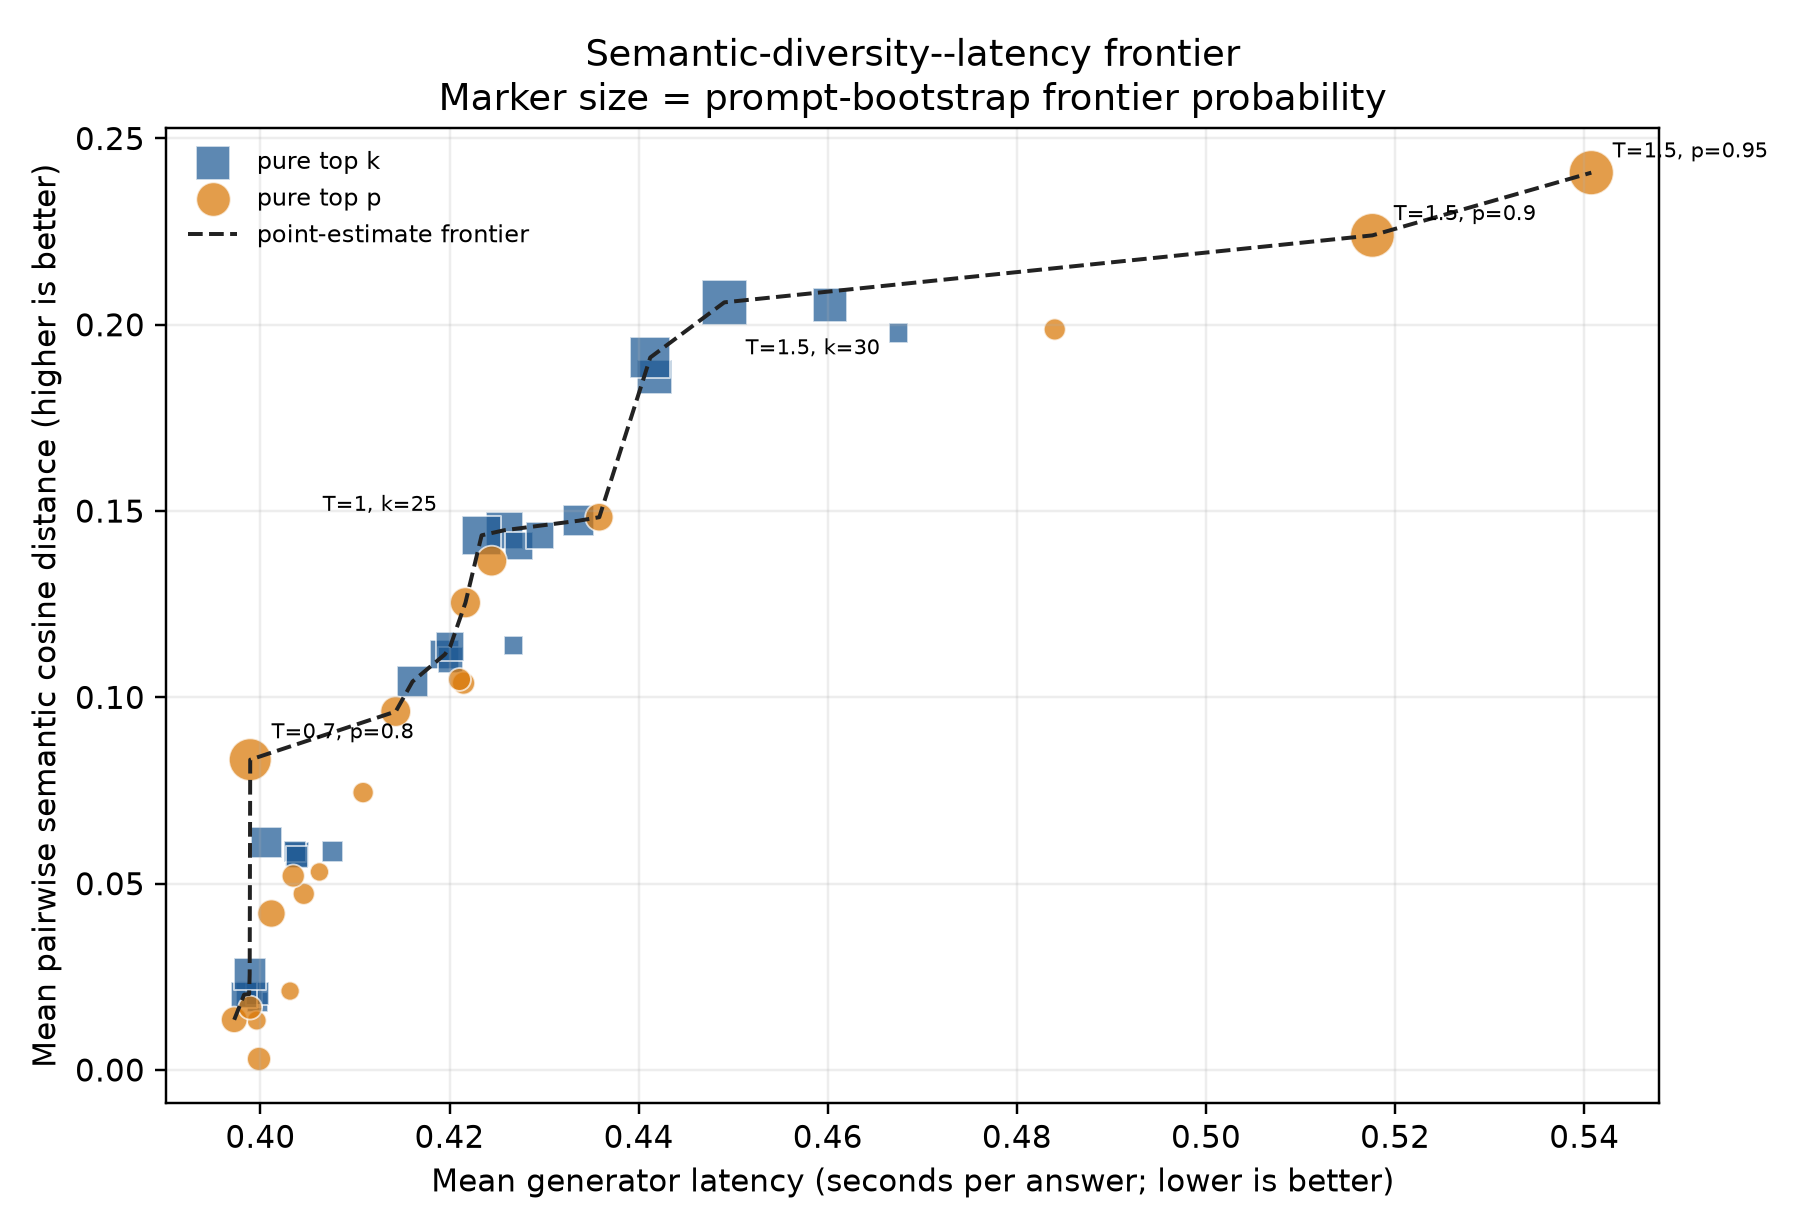
\includegraphics[width=0.78\linewidth]{semantic_diversity_latency_frontier.png}
\caption{Secondary semantic-diversity--latency Pareto analysis. Latency
differences are hardware-specific and mostly small in absolute magnitude.}
\label{fig:pareto}
\end{figure}

The four audited points were $T=0.7,p=0.8$ (0.3989 s), $T=1.0,k=25$
(0.4234 s), $T=1.5,k=30$ (0.4491 s), and $T=1.5,p=0.95$ (0.5407 s). Prompt
bootstrapping measures sensitivity to the question sample, not variation from
hardware state, job ordering, or repeated timing runs.

\section{Benjamini--Hochberg outcome families}
\label{app:bh-family}

The primary interaction correction was applied separately within the pure
top-$p$ and pure top-$k$ families to the same 13 outcomes:

\begin{enumerate}
\item mean correctness;
\item strict accuracy;
\item mean informativeness;
\item within-answer Distinct-1;
\item within-answer Distinct-2;
\item trigram repetition rate;
\item model generation latency;
\item generated-token throughput;
\item word length;
\item EOS stopping rate;
\item exact unique-answer rate;
\item pairwise token Jaccard distance; and
\item corpus Distinct-1.
\end{enumerate}

Corpus Distinct-2 was excluded from this family because it was undefined in
283 prompt-setting cells. The two embedding outcomes---semantic cosine
distance and semantic near-duplicate rate---were analyzed as a separate
two-outcome family.

\begin{thebibliography}{9}
\bibitem{lin2022truthfulqa}
Stephanie Lin, Jacob Hilton, and Owain Evans.
\newblock TruthfulQA: Measuring How Models Mimic Human Falsehoods.
\newblock \emph{Proceedings of ACL}, 2022.
\newblock \url{https://arxiv.org/abs/2109.07958}.

\bibitem{holtzman2020degeneration}
Ari Holtzman, Jan Buys, Li Du, Maxwell Forbes, and Yejin Choi.
\newblock The Curious Case of Neural Text Degeneration.
\newblock \emph{International Conference on Learning Representations}, 2020.
\newblock \url{https://arxiv.org/abs/1904.09751}.

\bibitem{zheng2023judge}
Lianmin Zheng et al.
\newblock Judging LLM-as-a-Judge with MT-Bench and Chatbot Arena.
\newblock \emph{Advances in Neural Information Processing Systems}, 2023.
\newblock \url{https://arxiv.org/abs/2306.05685}.

\bibitem{liu2016evaluate}
Chia-Wei Liu, Ryan Lowe, Iulian Serban, Mike Noseworthy, Laurent Charlin,
and Joelle Pineau.
\newblock How NOT To Evaluate Your Dialogue System: An Empirical Study of
Unsupervised Evaluation Metrics for Dialogue Response Generation.
\newblock \emph{Proceedings of EMNLP}, 2016.
\newblock \url{https://aclanthology.org/D16-1230/}.

\bibitem{reimers2019sentencebert}
Nils Reimers and Iryna Gurevych.
\newblock Sentence-BERT: Sentence Embeddings using Siamese BERT-Networks.
\newblock \emph{Proceedings of EMNLP-IJCNLP}, 2019.
\newblock \url{https://arxiv.org/abs/1908.10084}.

\bibitem{qwen25report}
Qwen Team.
\newblock Qwen2.5 Technical Report.
\newblock arXiv:2412.15115, 2024.
\newblock \url{https://arxiv.org/abs/2412.15115}.

\bibitem{qwen3report}
Qwen Team.
\newblock Qwen3 Technical Report.
\newblock arXiv:2505.09388, 2025.
\newblock \url{https://arxiv.org/abs/2505.09388}.

\bibitem{dettmers2023qlora}
Tim Dettmers, Artidoro Pagnoni, Ari Holtzman, and Luke Zettlemoyer.
\newblock QLoRA: Efficient Finetuning of Quantized LLMs.
\newblock \emph{Advances in Neural Information Processing Systems}, 2023.
\newblock \url{https://arxiv.org/abs/2305.14314}.
\end{thebibliography}

\end{document}
